\documentclass[UTF8,zihao=5,openany]{ctexbook}
\usepackage[paperwidth=170mm,paperheight=240mm,top=24mm,bottom=28mm,inner=26mm,outer=20mm,headheight=13pt,headsep=8pt,footskip=14pt]{geometry}
\usepackage{fontspec}
% 本地（Windows）用宋体 + Times New Roman；CI / Linux 下若缺字体则回落到 CTeX 默认（Fandol）
\IfFontExistsTF{Times New Roman}{\setmainfont{Times New Roman}}{%
  \IfFontExistsTF{Liberation Serif}{\setmainfont{Liberation Serif}}{}}
\IfFontExistsTF{Arial}{\setsansfont{Arial}}{%
  \IfFontExistsTF{Liberation Sans}{\setsansfont{Liberation Sans}}{}}
\IfFontExistsTF{Consolas}{\setmonofont{Consolas}}{%
  \IfFontExistsTF{Liberation Mono}{\setmonofont{Liberation Mono}}{}}
\IfFontExistsTF{SimSun}{\setCJKmainfont{SimSun}}{%
  \IfFontExistsTF{Noto Serif CJK SC}{\setCJKmainfont{Noto Serif CJK SC}[Language=Chinese Simplified]}{}}
\IfFontExistsTF{SimHei}{\setCJKsansfont{SimHei}}{%
  \IfFontExistsTF{Noto Sans CJK SC}{\setCJKsansfont{Noto Sans CJK SC}[Language=Chinese Simplified]}{}}
\IfFontExistsTF{SimSun}{\setCJKmonofont{SimSun}}{%
  \IfFontExistsTF{Noto Serif CJK SC}{\setCJKmonofont{Noto Serif CJK SC}[Language=Chinese Simplified]}{}}
\usepackage{xcolor}
\usepackage{titlesec}
\usepackage{tcolorbox}
\tcbuselibrary{skins}
\usepackage{booktabs,longtable,tabularx,array,multirow}
\usepackage{enumitem}
\usepackage{fancyhdr}
\usepackage[linktoc=all]{hyperref}
\usepackage{xurl}
\usepackage{needspace}
\usepackage{footmisc}
\renewcommand{\footnotelayout}{\raggedright}
% 分页处的节标题锚点：在标题真正落页之后再建锚点，避免目录跳到前一页
\makeatletter
\let\ttl@select@orig\ttl@select
\def\ttl@select#1#2#3#4{\ttl@select@orig{#1}{#2}{#3}{\phantomsection#4}}
\makeatother
\usepackage{graphicx}
\usepackage[font=small,labelfont=bf,labelsep=quad,margin=0.8cm]{caption}
\usepackage{amssymb}
\setlength{\parindent}{2\ccwd}
\usepackage{microtype}
\usepackage{tocloft}
\renewcommand{\cftchapfont}{\small\bfseries\color{ink}}
\renewcommand{\cftchappagefont}{\small\bfseries\color{ink}}
\renewcommand{\cftsecfont}{\small}
\renewcommand{\cftsecpagefont}{\small}
\setlength{\cftbeforechapskip}{7pt}
\setlength{\cftbeforesecskip}{1.5pt}
\renewcommand{\cftchapleader}{\color{teal!50}\cftdotfill{\cftdotsep}}
\let\cleardoublepage\clearpage
\widowpenalty=10000
\clubpenalty=10000
\definecolor{ink}{HTML}{16324F}
\definecolor{teal}{HTML}{0C7C86}
\definecolor{mint}{HTML}{EAF6F4}
\definecolor{sand}{HTML}{FFF6E5}
\definecolor{rose}{HTML}{FFF0F0}
\definecolor{gray}{HTML}{F4F6F8}
\hypersetup{colorlinks=true,linkcolor=teal,urlcolor=teal,citecolor=teal,pdftitle={把经历变成证据：计算机学生的四年规划与求职实战},pdfauthor={Sunday Xu},pdfsubject={计算机学生的四年规划与求职实战},pdfkeywords={计算机,秋招,求职,简历,面试,大学规划}}

\pagestyle{fancy}
\fancyhf{}
\fancyhead[LE,RO]{\footnotesize\color{ink!70}把经历变成证据}
\fancyhead[RE,LO]{\footnotesize\color{ink!50}计算机学生的四年规划与求职实战}
\fancyfoot[C]{\small\color{ink!80}\thepage}
\renewcommand{\headrulewidth}{0pt}
\makeatletter
\newif\ifbookappendix
\let\bookorigappendix\appendix
\renewcommand{\appendix}{\bookorigappendix\bookappendixtrue}
\newcommand{\chapterheadlabel}{\ifbookappendix 附录\thechapter\else 第\chinese{chapter}章\fi}
\makeatother
\titleformat{\chapter}[display]
  {\normalfont}
  {\color{teal}\fontsize{12pt}{15pt}\selectfont\bfseries\chapterheadlabel}
  {10pt}
  {\color{ink}\fontsize{22pt}{28pt}\selectfont\bfseries}
  [{\vspace{12pt}\color{teal!55}\rule{4.2cm}{2pt}}]
\titlespacing*{\chapter}{0pt}{-14pt}{12pt}
\titleformat{\section}{\large\bfseries\color{ink}}{\textcolor{teal}{\thesection}}{0.65em}{}
\titlespacing*{\section}{0pt}{1.6ex plus .3ex minus .2ex}{0.8ex plus .1ex}
\titleformat{\subsection}{\normalsize\bfseries\color{teal}}{\thesubsection}{0.6em}{}
\setlist[itemize]{leftmargin=2.2em,itemsep=2pt,topsep=3pt}
\setlist[enumerate]{leftmargin=2.4em,itemsep=3pt,topsep=3pt}
\newcolumntype{Y}{>{\raggedright\arraybackslash}X}
\newcommand{\stage}[1]{\textcolor{teal}{\textbf{#1}}}
\newcommand{\evidence}[1]{\textcolor{teal}{\textbf{【证据：#1】}}}
\newcommand{\todo}[1]{\textcolor{red}{\textbf{【待补：#1】}}}
\newtcolorbox{keybox}{colback=mint,colframe=teal,boxrule=0.7pt,arc=2mm,left=3mm,right=3mm,top=2mm,bottom=2mm}
\newtcolorbox{warningbox}{colback=sand,colframe=orange!70!black,boxrule=0.7pt,arc=2mm,left=3mm,right=3mm,top=2mm,bottom=2mm}
\newtcolorbox{casebox}{colback=gray,colframe=ink!45,boxrule=0.5pt,arc=2mm,left=3mm,right=3mm,top=2mm,bottom=2mm}
\newtcolorbox{toolbox}{colback=white,colframe=teal!70!black,boxrule=0.8pt,arc=2mm,left=3mm,right=3mm,top=2mm,bottom=2mm}
\setcounter{tocdepth}{1}
\setcounter{secnumdepth}{3}
% 留言板条目：\boardentry[color=…, size=12pt, font=\bfseries, indent=2cm, rotate=-2]{署名}{时间}{内容}
\pgfkeys{/board/.is family, /board/.cd,
  color/.initial=ink,
  size/.initial=10.5pt,
  font/.initial=\normalfont,
  indent/.initial=0pt,
  rotate/.initial=0,
  gap/.initial=2pt}
\newcommand{\boardentry}[4][]{%
  \begingroup
  \pgfkeys{/board/.cd,#1}%
  \par\vspace{\pgfkeysvalueof{/board/gap}}%
  \noindent\hspace*{\pgfkeysvalueof{/board/indent}}%
  \rotatebox{\pgfkeysvalueof{/board/rotate}}{%
    \parbox[t]{\dimexpr\linewidth-\pgfkeysvalueof{/board/indent}\relax}{%
      \pgfkeysvalueof{/board/font}%
      \fontsize{\pgfkeysvalueof{/board/size}}{\dimexpr\pgfkeysvalueof{/board/size}*6/5\relax}\selectfont
      \color{\pgfkeysvalueof{/board/color}}%
      #4\enspace{\scriptsize\color{ink!45}#2 · #3}}}%
  \par
  \endgroup}
% 填写线：从当前位置一直画到行尾/盒内右边界
\newcommand{\fillrule}{\leavevmode\leaders\hbox{\rule[-0.15em]{2pt}{0.4pt}}\hfill\kern0pt}
\begin{document}
\begin{titlepage}
\thispagestyle{empty}
\centering
\vspace*{0.6cm}
\noindent{\color{teal!70}\rule{\textwidth}{0.5pt}}\par
\vspace{2.6cm}
{\fontsize{34pt}{44pt}\selectfont\bfseries\color{ink} 把经历变成证据\par}
\vspace{0.9cm}
{\large\color{teal} 计算机学生的四年规划与求职实战\par}
\vspace{1.2cm}
{\color{teal!55}\rule{5.5cm}{2pt}}\par
\vspace{2.4cm}
\begin{tcolorbox}[colback=mint,colframe=teal,width=0.88\textwidth,boxrule=0.8pt,arc=3mm]
\centering\normalsize
把学习变成证据，把选择变成实验，\\[2pt]
把工作变成下一次选择的起点。
\end{tcolorbox}
\vfill
{\small\color{ink} 工作稿 v1.0\qquad 2026 年 11 月\par}
\vspace{0.5cm}
\noindent{\color{teal!70}\rule{\textwidth}{0.5pt}}
\end{titlepage}
\thispagestyle{empty}
\vspace*{3cm}
\begin{center}
{\large\bfseries 把经历变成证据}\\[0.2cm]
{\normalsize 计算机学生的四年规划与求职实战}\\[1.6cm]
{\normalsize Sunday Xu 著}\\[0.2cm]
{\normalsize 工作稿 v1.0}\\[0.3cm]
{\normalsize 2026 年 11 月}\\[2.2cm]
{\small 反馈与勘误：X \url{https://x.com/sundayai_}\quad 邮箱 \url{sunday.xu@ttcadvisory.com}}\\[1.2cm]
{\footnotesize 本书为工作稿，未经终审、版权清理与事实核验，不作为出版定稿流通。}
\end{center}
\clearpage
\frontmatter
\thispagestyle{empty}
\vspace*{1.2cm}
\noindent\noindent{\color{teal!70}\rule{\textwidth}{0.5pt}}\par
\vspace{1.4cm}
{\Large\bfseries\color{ink} 作者}\par
\vspace{0.8cm}
{\large Sunday Xu（X：@sundayai\_）}\par
\vspace{1.2cm}
\begin{minipage}{0.86\textwidth}
\small
计算机大类本科。参加过数学建模与人工智能方向的比赛，做过数据工程与 AI 应用的实习，长期在 X 上写计算机学生的专业选择与求职。这本书里的案例，一半来自他自己踩过的坑，一半来自他访谈过的同学、学长和面试官。

\medskip
他的判断很朴素：与其反复讨论“该选什么”，不如去做一个成本可承受的小实验，然后把结果记下来。书里所有的方法，都可以压缩成这一句。
\end{minipage}
\vfill
\noindent{\color{teal!70}\rule{\textwidth}{0.5pt}}
\clearpage

\clearpage
\chapter*{序：在他人的影响中，成为自己}
\phantomsection\addcontentsline{toc}{chapter}{序：在他人的影响中，成为自己}

这本书最初只有二十三页。2026 年秋天，我把写给学生看的笔记整理成一个薄薄的 PDF，发给几个刚入学的朋友。他们的回应很直接：道理都对，但我还是不知道下周该做什么。于是有了第二版、第三版。每一次修订几乎都是被具体的追问推着走的：绩点和项目怎么平衡、夏令营要不要去、简历上写“参与”到底算不算证据。

修订的过程中我一直在想一个问题：人究竟是怎么成为自己的。回头看近八年，几个关键的路口背后都站着别人。我想把这些写下来，因为如果你刚进大学、还不知道要往哪走，我想先告诉你：写这本书的人，也曾经完全不知道。

\section*{一、我们总是在有限的认知里，选看起来最好的答案}

初中时我化学成绩不错，但具体为什么比同学好，我并不清楚，只是卷子上总有不少红勾，老师也常在课堂上表扬我。有一次她半开玩笑地说，你化学这么好，以后可以考虑当科学家。我信了。那时候我对科学家的理解很简单：穿白大褂，在实验室里做实验，发现一些了不起的东西，于是开始觉得自己该往化学走。到高中，我第一次认真考虑就业。当时“生化环材”就业难的讨论已经很多，我意识到不能因为一门课成绩好就决定未来几十年的方向。

有一次职业规划课，老师让我们各自找一个职业，查资料、上台介绍。其他同学大多选了律师、教师、厨师，我在网上翻资料时偶然刷到“大数据工程师”，觉得这个名字有意思，就花了不少时间准备。上台时老师问了不少问题，我大多答了出来。那是我第一次意识到，除了自己熟悉的职业，还有很多我此前根本不知道的工作。后来填志愿，父母希望我选层次更高的学校，但专业不是我感兴趣的方向，我拒绝了，选了数据科学与大数据技术。现在回头看，这个决定谈不上高瞻远瞩，它只是当时的我，在有限的信息里经过有限的思考作出的选择。但我不因此否定当时的自己——那时候的我，确实只能看到那么远。

\section*{二、进入大学以后，我反而比高中更迷茫}

刚入学时我对数据科学抱有不少期待，以为会接触大量数学、统计学和机器学习；真正开始学之后，发现培养方案和自己的预期有不小的差距。身边的同学似乎都有目标：有人卷绩点，有人准备入党，有人参加竞赛和学生组织，有人早早准备考研。我却经常坐在图书馆里，反复搜索“数据科学本科毕业能做什么”“机器学习和计算机科学该选哪个方向”，甚至逼自己去读根本不感兴趣的论文。那时候大模型已经开始快速发展，但我对它的理解非常浅薄，只觉得它是一个能聊天、能写文章的工具，没有意识到 Transformer 所代表的技术体系正在改变整个软件行业。

直到我遇到一位研究机器学习的学长。他从 Python 语法开始教我，一点点带我接触机器学习、神经网络。第一次真正理解 Transformer 时，我有一种很奇妙的感觉：输入一串文本，经过矩阵运算、注意力机制和层层变换，最终涌现出复杂的理解与生成能力。后来我又认识了一位在中科院自动化所读博的网友。我当时在找实习，他告诉我，如果暂时找不到公司实习，也可以先去科研团队积累经验，还建议我联系老师申请科研实习。于是我发了邮件，开始接触科研。如果没有这两个人，我可能还在各种职业介绍、考研目录和就业分析之间反复打转；他们没有替我决定未来，但确实让我看到了此前不知道的可能性。

\section*{三、真正让我不再迷茫的，是第一次进入真实的工作环境}

后来我开始找公司的实习，面试并不顺利，有些技术问题答不上来，有些在现在看来只是基础的工程知识，但最终我还是通过了。现在我也不确定当时是什么让面试官决定录用我：可能是项目，可能是学习潜力，也可能只是综合判断。进入公司之后，我才发现学校和企业是两套逻辑。学校里题目已经给出、要求已经明确，按评分标准提交结果；公司里领导只说要实现什么业务功能，怎么设计、怎么拆模块、怎么处理异常、怎么和其他系统交互，都要自己想。代码能跑并不意味着任务完成，还要考虑开发规范、稳定性、权限控制、日志审计、异常处理和后续维护；更重要的是理解业务人员真正想解决什么，而不是照着对方描述的文字机械地敲代码。

我开始接触 AI 应用开发，尝试把大模型、Agent、工具调用融进真实业务，工作之余把能公开的项目整理到开源平台。渐渐地我发现，学校里很难获得的东西，工作中能快速积累：开发速度、工程规范、业务理解和沟通。最有成就感的一次，是参与开发的成果被公司整理成专利和软件著作权申请材料。看到自己写过的代码变成一份正式的技术材料时，我第一次具体地意识到，我掌握的知识真的可以在现实里创造价值。这和考试考了多少分、参加了多少比赛，是完全不同的体验。

\section*{四、几乎每一次成长，背后都有别人的身影}

把经历连起来看，会发现一个有意思的现象：初中是化学老师的表扬让我产生了科学家的想象，高中是职业规划课让我知道了大数据工程师，大学是学长带我入门深度学习，后来是那位博士网友介绍科研实习，进入公司是领导愿意给我机会，再后来是法务、律师和同事帮我完成此前完全不了解的事。我曾经以为自己是靠一系列独立选择走到今天的，现在发现，每当我进入一个新阶段，总有人在某个节点为我打开一扇门。

这让我产生了一个疑问：我的选择究竟是自我的觉醒，还是被环境裹挟着向前。如果没遇到那位学长，我还会接触深度学习吗；如果公司没有录用我，我还会在这个时间点获得这些工程经验吗。这些问题没有答案，但我逐渐意识到，我们常常高估个人意志的作用，却低估他人、环境和偶然性提供的帮助。当然，这不意味着努力不重要。别人可以教我 Python，但不能替我写完代码；可以给我实习机会，但不能替我完成项目。所以我现在更愿意这样理解：别人为我打开了门，但走不走进去、走进去之后怎么行动，仍然是我自己的事。

\section*{五、成长并不意味着所有变化都是好的}

这几年我确实成长了不少，但也发现自己身上出现了一些不太好的变化。以前父母知道我要去外地实习会担心，甚至争吵，我多半默默听着；现在我学会了安抚他们的情绪，说一些能让他们放心的话，有时候甚至承诺毕业前都待在学校，实际上已经开始找下一段实习。我也越来越习惯向他们隐瞒自己的生活：好消息会被拿去炫耀，坏消息会变成教育我的理由。与其解释，不如不说。这保护了我的私人空间，但我也意识到，自己正在习惯用“管理别人的预期”来减少冲突。

还有一件事我印象很深。有一次领导让我帮忙找实习生，我在几个平台发了信息，说简历可以直达部门负责人。收到简历后，我发现不少人工程经历比较单薄，就没有转交，却告诉部分求职者已经帮他们转发了。当时的想法很简单：什么都往上报，会显得自己没认真筛。现在回头看，这件事不值得自我辩护。我有权筛选和拒绝推荐，但没必要用虚假的承诺维护自己的职业形象。

人在成长中，不只会获得知识和能力，也可能学会隐瞒、操纵信息，以及利用信息差获取便利。我们常把成熟理解为越来越懂规则、越来越会处理关系，但成熟也可能带着一些不那么好的东西：一个人可以越来越有能力，却不一定越来越诚实。我还没有完全解决这些问题，只是开始意识到，在获得更多能力和选择权之后，自己也要承担更多责任。

\section*{六、如果重新走一遍，我还是愿意一边选择，一边感受}

现在如果有人问我，大学生究竟该怎么规划未来，我很难给出标准答案，因为我自己就反复改过方向：初中想当科学家，高中担心专业就业，大学研究考研方向，后来接触机器学习，再到今天做 AI 应用开发。如果每个阶段的我都必须提前确定未来十年的路线，我大概会一直焦虑。我也曾因为身边人都在考研、卷绩点、打比赛，怀疑自己是不是走错了路。

后来我逐渐明白，不同的人有不同的目标：有人适合科研，有人适合工程，有人想进体制，有人想去企业。绩点、竞赛、学生组织、实习、科研这些东西本身没有绝对的好坏，重要的是它们能否帮你实现真正想要的目标。我不认为所有大学生都该像我一样把大量时间投在实习和工程实践上，也不认为必须尽早找到所谓的热爱。有些事情只有真正接触之后才知道喜不喜欢，有些能力只有在真实环境里才发现自己有没有，有些选择也只有走过一段路才能判断适不适合。

\section*{七、你不必急着成为一个已经确定的人}

如果你刚刚进入大学，正在为专业、考研、就业、科研感到迷茫，我想告诉你：你不必在大一就知道自己未来要成为谁，就像看到别人提前交卷，也没有必要急着交卷。你可以先认真学一门课，参加一次科研活动，做一个自己感兴趣的项目，尝试一段实习，认识一些和你有不同经历的人。你可能会发现自己喜欢原本不感兴趣的领域，也可能发现曾经向往的事情并不适合自己，这都没有关系。不要因为别人已经有了明确的规划，就认为自己落后了；也不要因为某个领域暂时热门，就觉得自己必须进去。

你可以听取建议，也可以接受帮助；可以走一段大家都在走的路，也可以在了解之后选择一条不同的路，但请尽量保留独立判断的能力。还有一点：不要把人生变成一场不断向别人证明自己的考试。你不需要通过考上更好的学校、进入更好的公司、拿到更高的薪水，来证明自己值得被认可。职业发展很重要，个人能力很重要，但它们不是一个人全部的价值。人的一生可能并不是寻找一个早已存在的、正确的自我，而是在一次又一次的接受、拒绝、尝试、妥协与重新选择中，逐渐成为自己。别人为你打开了门，不代表你是被推着走进去的；你最终会成为怎样的人，也不必由今天的你提前给出答案。

\vspace{0.4cm}
\noindent\hfill —— 2026 年 11 月

\clearpage

\chapter*{写给读者：这本书怎么用}
\phantomsection\addcontentsline{toc}{chapter}{写给读者：这本书怎么用}
如果你还没有进入大学，你可能正在问：应该选什么专业，哪所学校更好，计算机是不是已经太卷。

如果你刚刚入学，你可能正在问：绩点、竞赛、学生组织、课程、项目和实习，到底应该把时间放在哪里。

如果你已经读到大二或大三，你可能正在问：我是不是学得太杂了，应该什么时候收敛，怎样做出能被看见的作品。

如果你正在秋招，你可能正在问：简历怎么写，面试怎么讲，拿到几个 offer 以后怎样判断哪家公司值得去。

这本书不替你回答一个永远正确的“应该”。它只提供一套更可靠的工作方式：先把问题说清楚，做一个成本可承受的实验，进入真实环境，记录结果，再根据证据调整方向。

书里的第一人称，都是我自己的经历：转专业、比赛烂尾、实习、被拒。细节做过脱敏，情境是真的。它们是经验材料，不是普遍定律。涉及行业数字和薪资的地方，我尽量给出可查的依据；查不到的就直说不知道，而不是编一个听起来合理的数。

\begin{keybox}
\textbf{本书的核心承诺：}帮助你把“我想学点什么”逐步转化为“我做过什么、解决过什么问题、能为哪类岗位提供什么证据”。

\textbf{本书不承诺：}保证 offer、保证薪资、保证某个热门方向永远正确，也不替你承担选择的后果。
\end{keybox}

这本书仍在修改。如果你发现事实错误、过期的数据，或者某条建议在你的学校、地区、家庭条件下根本不成立，欢迎告诉我。

X：\url{https://x.com/sundayai_}　邮箱：\url{sunday.xu@ttcadvisory.com}。涉及数据、引用和授权的问题，请注明页码与原文，我会逐条核对。

\section*{如何使用本书}
\phantomsection\addcontentsline{toc}{section}{如何使用本书}

\begin{center}
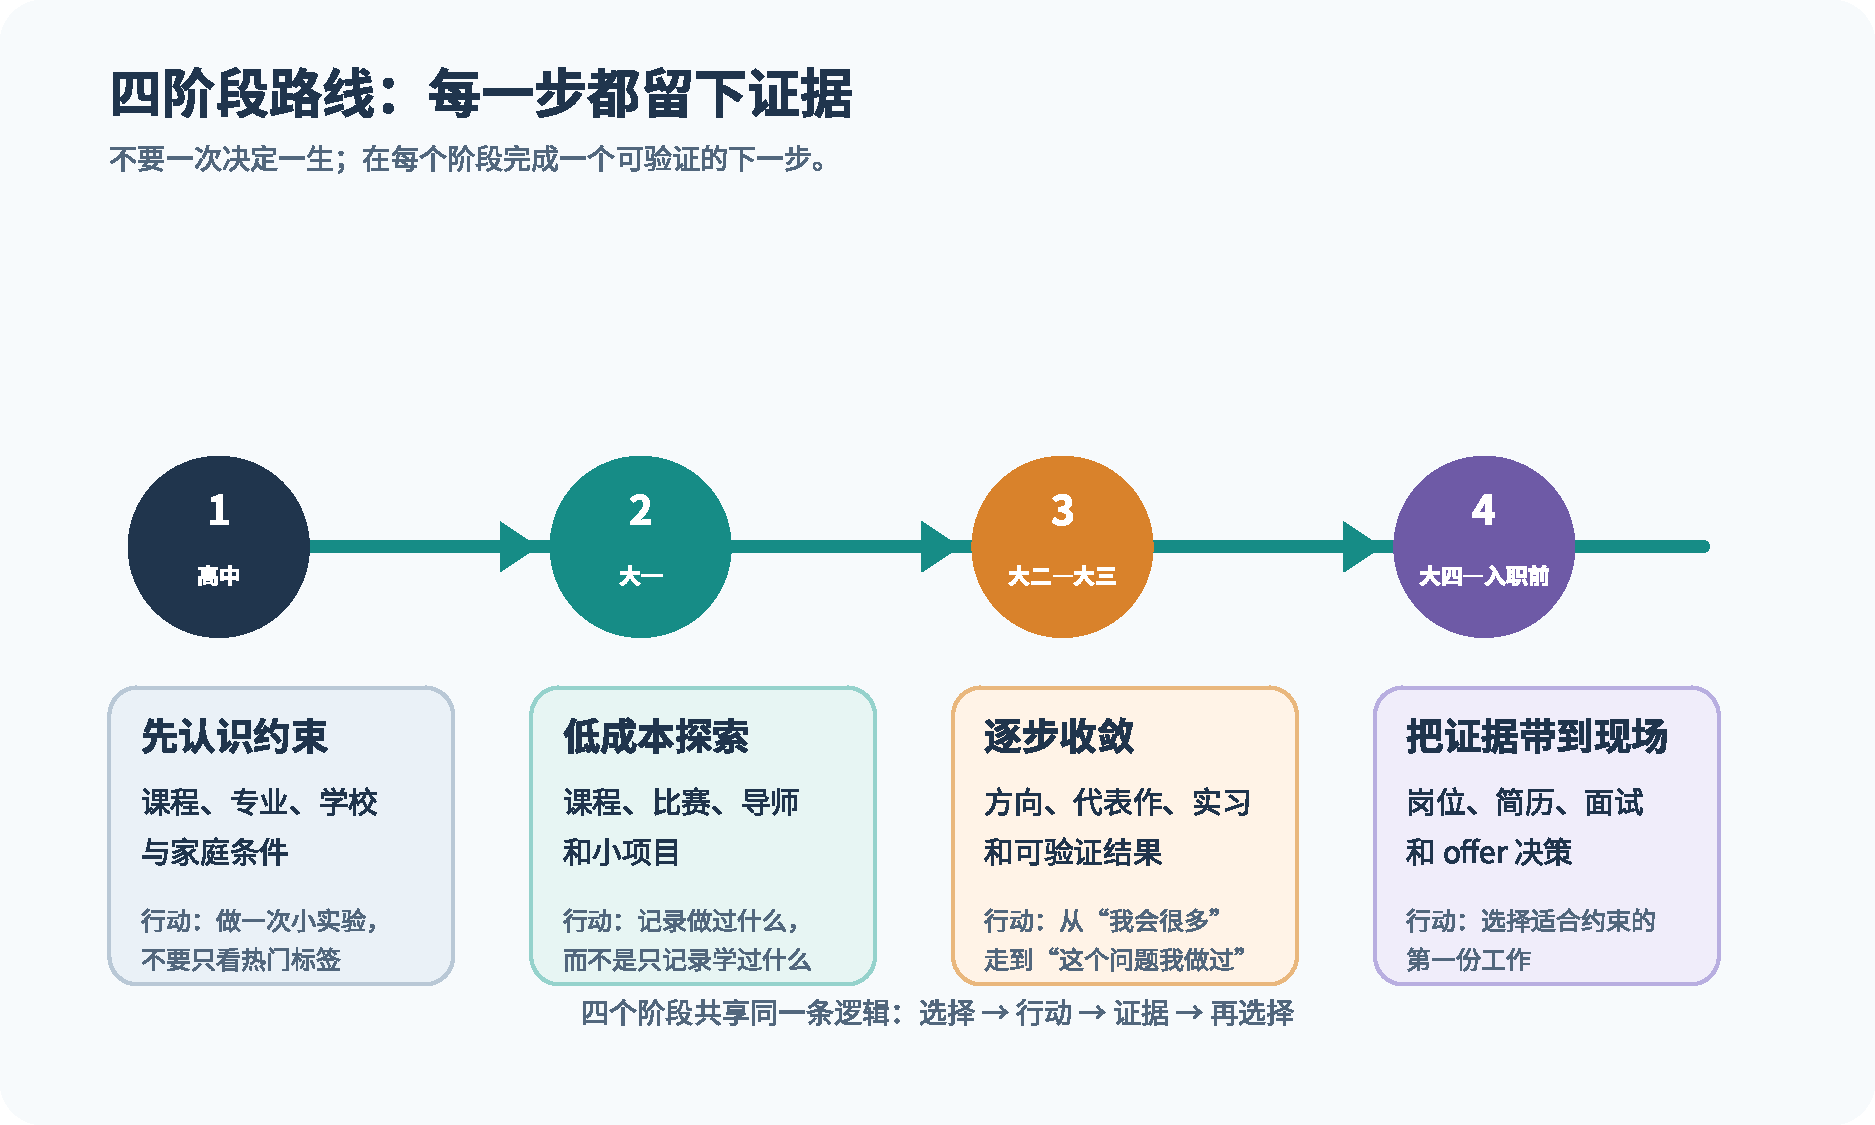
\includegraphics[width=0.95\textwidth]{assets/pdf/four_stages.pdf}
\par\nopagebreak\smallskip
\captionof*{figure}{卷首图：四类读者共享的一条成长路线，从理解起点到形成证据}
\end{center}

这本书不用从头读到尾。它按“你现在卡在哪”来组织，先读和你处境相关的那几章，其余的需要时再翻。

\begin{itemize}
\item \textbf{高中生、刚报完志愿}：第 1--2 章。看懂专业、课程和岗位的关系，知道四年怎么走、哪里会走错。
\item \textbf{大一}：第 1--4 章。看清时间轴，把基础打稳，做第一个有人用的东西。
\item \textbf{大二}：第 3--7 章。工程能力、刷题、协作、收敛方向，同时开始看岗位和企业。
\item \textbf{大三}：第 2、4、5、7--11 章。时间轴、分叉口、刷题、机会、简历面试、秋招与实习。
\item \textbf{大四}：第 9--11 章。秋招节奏、从分层市场到第一家公司、实习转正与入职。
\item \textbf{心态崩了的时候}：先读第 12 章，再回来看别的。
\end{itemize}

章节之间不是线性依赖。每章基本按“一个场景、一个方法、一个反例、一个能立刻做的动作”写，工具类的章节会直接给表格和模板，照着填就行。

书里的案例标注了来源，正文里能标的地方都标了：
\begin{itemize}
\item \textbf{【作者经历】}——我自己踩过的坑，细节做过脱敏。
\item \textbf{【示例】}——为了说明一个方法而构造的情形，不是真实案例，也不假装是。
\item 公开数据与报告在脚注和附录 F 里给出出处，可以按图索骥。
\end{itemize}

没有标来源的行业数字，请当作待验证的假设。这本书的原则是：观点可以带立场，事实必须能追溯。

也要说清样本的边界：书里的案例主要来自作者所在的学校、城市和行业，偏向互联网与 AI 方向，缺少双非院校、专科、西部高校、家庭经济困难、身体障碍等样本。凡涉及“大多数人如何”的判断，请把它当成待验证的假设，而不是统计结论。

\clearpage
\tableofcontents
\clearpage
\listoffigures
\clearpage
\listoftables
\mainmatter
\clearpage\chapter{从问题出发：先决定要解决什么，再选专业}
\section{不要在信息不足时假装已经知道答案}
很多学生在入学前就想把未来十年决定下来。他们会比较学校层次、城市、专业名称和就业率，然后试图从一张表里找到唯一正确的选择。

这样做的问题不是搜集信息，而是把选择误解成一次性的预测。你无法在高中阶段知道自己三年后会喜欢什么技术，也无法知道某个岗位在毕业时的具体名称。你能做的是减少纠偏成本：理解课程，查看岗位，和真实的人交流，做小规模尝试。

\begin{casebox}
\textbf{【作者经历】}我初中化学成绩不错，老师夸得多，就以为自己要当科学家；高中听说“生化环材是天坑”，立刻掉头找别的出路；报志愿时看到“数据科学可以在很多领域赋能”，就报了它。真正入学后我才发现，培养方案里大半是我提不起兴趣的课，于是开始自己找方向——那两年我一直在搜“这个专业以后能干什么”，逼自己看文献，效果很差。直到大模型和 Agent 工具出现，我开始做项目、找实习，才第一次知道自己能为企业解决什么。回头看，问题不在于选错专业，而在于我在信息最少的时候，要求自己做一个最终决定。
\end{casebox}

一个选择是否合理，要看三个条件：
\begin{enumerate}
\item 当时掌握的信息是否足够支持这个决定；
\item 这个决定是否留下了纠偏和再选择的空间；
\item 你是否设置了可以观察结果的时间点。
\end{enumerate}

\section{把“我想学 AI”改写成可验证问题}
“我想学 AI”不是一个行动计划。它至少可以被改写成四种不同的问题：
\begin{itemize}
\item 我想进入哪类岗位：开发、算法、数据、测试、产品技术还是研究？
\item 我想解决哪类问题：推荐、搜索、信息抽取、智能客服、评测、可靠性还是工具调用？
\item 我需要什么证据：课程成绩、竞赛、论文、开源、项目上线、业务指标还是实习反馈？
\item 我能在四到八周内做什么实验，判断自己是否愿意继续？
\end{itemize}

\begin{toolbox}
\textbf{方向实验卡}

方向：\fillrule

我对它的初始假设：\fillrule

两周内可以完成的最小实验：\fillrule

结果如何观察：\fillrule

继续的条件：\fillrule

退出或转向的条件：\fillrule
\end{toolbox}

\section{选择评价体系，而不是机械跟随评价}
绩点、竞赛、学生组织、项目和实习不是同一种货币。它们能证明的事情不同：绩点可以证明你在课程评价体系中的稳定性；竞赛可以证明你在有限时间里解决问题和协作的能力；项目可以证明你是否把东西做出来；实习可以提供真实组织中的交付证据。

它们不能随意互相替代。一个开发岗位可能更重视上线系统和工程责任，一个研究岗位可能更重视高质量论文和实验设计。真正的问题不是“哪个最有用”，而是“这个岗位需要我证明什么”。

\begin{warningbox}
不要把反主流本身当成独立思考。机械卷绩点是一种从众，机械鄙视绩点也可能是另一种从众。评价标准应该由目标、约束和证据决定。
\end{warningbox}


还有一个更隐蔽的从众：把选拔规则当成人生规则。高考用一套分数把人排成序，进大学以后很多人继续用同一套逻辑判断一切——绩点高就是方向对，排名靠前就是能力强。可评分机制只在一个窗口内有效：毕业那天，那串分数就作废了。更值得问的是，这套评价正在训练我什么能力，它两年后还有没有用。\footnote{《上海交通大学学生生存手册》“失败的思维方式·高考思维”，\url{https://github.com/1638410/SurviveSJTUManual/blob/master/li-zhi-pian/shi-bai-de-si-wei-fang-shi/gao-kao-si-wei.md}。}另一层是“被动思维”：上课、考证、参加活动，很多人是被推着走的，说不出为什么做。如果一门课你自学效率更高、它也不在你的目标路径上，那“去上课”本身就是个需要解释的决定。\footnote{同上，“失败的思维方式·被动思维”，\url{https://github.com/1638410/SurviveSJTUManual/blob/master/li-zhi-pian/shi-bai-de-si-wei-fang-shi/bei-dong-si-wei.md}。}

\section{计算机大类里到底有哪些专业}

\subsection{先看课程表，别先看专业名}
“计算机科学与技术”和“软件工程”在招生目录上只差几个字，四年后能做的事却不一样。这种差别很少写在专业介绍里，它写在培养方案的课程表和学分要求里。

一句可以操作的话：专业之间的差别主要在三处——数学与硬件的比重、工程实践的比重、高年级方向课的自由度。你不需要在报志愿前看懂整份培养方案，但至少要看四件事：数学课有多少学分、大三下到大四的主干课是什么、实践环节占多少、转专业和大类分流的规则怎么写。

\needspace{9\baselineskip}
\subsection{六个常见专业，差在什么地方}
\needspace{5\baselineskip}
\captionof{table}{六个常见专业，差在什么地方}
\begin{center}\footnotesize
\begin{tabularx}{\linewidth}{p{0.16\linewidth}p{0.26\linewidth}p{0.22\linewidth}Y}
\toprule
专业 & 课程重心 & 典型去向 & 容易被忽略的坑 \\
\midrule
计算机科学与技术 & 数学、算法、编译、体系结构、操作系统 & 读研、算法岗、后端、基础设施 & 课程偏理论，不主动做项目会“什么都会一点” \\
软件工程 & 工程化、软件过程、前后端、测试与质量 & 开发岗、测开、产品技术 & 部分学校把它当“低配计科”，基础课被压缩 \\
人工智能 & 机器学习、深度学习、概率与优化 & 算法岗、AI 工程、读研 & 本科容易停在调包，系统课和工程课偏少 \\
数据科学与大数据 & 统计、数据库、分布式、数据工程 & 数据开发、数据分析、算法 & 岗位名称混乱，常被误当成“算法预备班” \\
网络空间安全 & 密码学、系统安全、网络攻防 & 安全岗、运维、合规 & 偏攻防，开发能力要自己补 \\
电子信息／自动化（常与计算机混报） & 电路、信号、嵌入式、控制 & 嵌入式、硬件、自动驾驶 & 编程训练少，转纯软件要补大量基础 \\
\bottomrule
\end{tabularx}
\end{center}

这张表只能用来提问，不能用来下结论。同一个专业在不同学校的课程表差别，往往比专业名称之间的差别更大。所以真正该干的事是：拿到你想去的三所学校的培养方案，逐条对照。

了解专业不能只靠搜索。更可靠的信息来自三类人：系里的青年教师（知道这个方向最近在做什么）、高年级学生和研究生（知道课程和出路的真实样子）、来校宣讲的工程师（知道岗位要什么）。同时要过滤过时的经验——五年前的路，今天可能已经不通了。\footnote{《上海交通大学学生生存手册》“你想要做什么”一节列了更细的信息渠道，并提醒“十年甚至五年前的人的路往往不再适用于你”。\url{https://github.com/1638410/SurviveSJTUManual/blob/master/li-zhi-pian/ben-ke-si-nian-yao-zuo-shen-me.md}。}

收入排序也在变。麦可思《2026 年中国本科生就业报告》里，月收入前十中出现了微电子科学与工程、电子科学与技术、自动化、光电信息科学与工程四个工科专业，计算机科学与技术、软件工程则跌出前十\footnote{麦可思研究院《2026 年中国本科生就业报告》（2026 年 6 月）；本稿未获全文，数字本稿未见原始报告全文，转引自 TechWeb 2026 年 7 月 6 日报道，引用前请核对原报告；具体榜单与口径以原报告表格为准。}。这不代表计算机不行了，而是“只要是计算机就高薪”的假设不再成立——专业之间的差别，越来越取决于你最终进了哪条产业链。

\subsection{怎么读一份培养方案：四步}
\begin{enumerate}
\item \textbf{数必修学分。} 数学（高数、线代、概率统计）一共多少学分，占比多少。数学课多的专业，读研和算法方向更顺；数学课少的专业，不是不能做算法，而是你要自己补。
\item \textbf{找高年级主干课。} 大三下到大四的必修与限选课，才是决定你能不能碰真实系统的部分。如果高年级全是选修、靠学生自己拼，说明这个方向要靠你主动补。
\item \textbf{看实践环节。} 课程设计、生产实习、毕业设计各占多少学分，是“交个报告”还是“真的要跑起来”。
\item \textbf{看规则。} 大类分流按什么排序（绩点、志愿还是考试）、转专业名额多少、保研率与加分细则、奖学金与挂科重修的规定。这些规则会直接决定你后三年的策略。
\end{enumerate}

举个读法示范。假设某份方案里，“数据结构”排在大二上，“操作系统”在大三上，“数据库”在大三下，而“编译原理”和“分布式系统”在大四。那么你在申请暑期实习的大三下 2--4 月时，分布式和编译还没学过——这两门课就不能写进简历，面试也不会问；你该拿来展示的是数据结构、操作系统、数据库和那门课程设计。反过来，如果某校把操作系统和数据库都压在大三上，你就要在投暑期实习前，用一个学期把这两门课的项目做扎实。

\subsection{被调剂到了不喜欢的专业怎么办}
先算清楚三件事：转专业的窗口和条件、辅修或微专业的可能、自学路线的成本。多数学校的转专业窗口在大一结束，条件通常是绩点排名加笔试面试；辅修的含金量低于转专业，但能补齐课程名。

如果转不了，也不必重读。计算机这一行筛人时看的是“你做过什么”，不是“你毕业证上印的哪个专业名”。把本专业的课修到不挂，把多余的时间投到项目和实习上，是最常见的解法；前提是你要比科班的人多补几门课（数据结构、操作系统、数据库、网络），而且要在大二结束前补完。

\subsection{练习：三张表}
三张表各管一件事：课程翻译表把课程翻译成真实问题，专业对照表比较你现在的起点和目标，专业决策卡写下你的约束。

课程的价值不在于分数，而在于它能不能被翻译成真实问题。每学完一门主干课，填一行：

\begin{toolbox}
\needspace{5\baselineskip}
\captionof{table}{课程翻译表}
\begin{center}\small
\begin{tabularx}{0.94\linewidth}{p{0.18\linewidth}p{0.24\linewidth}p{0.24\linewidth}Y}
\toprule
课程 & 一个真实问题 & 一个小项目 & 仍然不懂的概念 \\
\midrule
数据结构 & & & \\
操作系统 & & & \\
数据库 & & & \\
计算机网络 & & & \\
概率统计 & & & \\
\bottomrule
\end{tabularx}
\end{center}
\end{toolbox}

\textbf{专业对照表。}

\begin{toolbox}
\needspace{5\baselineskip}
\captionof{table}{专业对照表}
\begin{center}\small
\begin{tabularx}{0.92\linewidth}{p{0.16\linewidth}YYY}
\toprule
 & 我的专业 & 目标专业 & 目标岗位要求的专业 \\
\midrule
数学与基础课学分 & & & \\
高年级主干课 & & & \\
实践环节占比 & & & \\
转专业／保研规则 & & & \\
\bottomrule
\end{tabularx}
\end{center}
\end{toolbox}

\textbf{专业决策卡。}

\begin{toolbox}
最想避免的三种学习内容：\fillrule

愿意连续投入两年的基础能力：\fillrule

家庭与地域限制：\fillrule

三个可接受的替代路线：\fillrule

两周内要验证的一个未知：\fillrule
\end{toolbox}

\chapter{大学四年：时间轴、弯路与第一个分叉口}
\section{秋招不是大四才开始的}
很多人的秋招，实际上在大三下学期的二月就结束了。

2026 届全国普通高校毕业生规模预计 1270 万人，同比增加 48 万\footnote{教育部：2026 届全国普通高校毕业生规模预计 1270 万人，同比增加 48 万（新华社，2025 年 11 月 20 日）。}。在这样的规模下，“什么时候投”往往比“投多少份”更决定结果。

原因很简单：大厂和中厂的核心岗位，大部分名额在暑期实习转正阶段就被消耗掉。暑期实习的投递窗口通常在大三下 2--4 月，笔试面试在 3--5 月，实习在 7--9 月，转正答辩在 8--9 月。等到大四的九月正式批开始，剩下的多是补招名额和竞争更激烈的岗位。

所以时间轴要倒着排：想在 2027 年 9 月拿到 offer，就要在 2027 年 2--3 月投暑期实习；想在 2027 年 2 月拿出简历，就要在 2026 年 12 月前有项目和一段经历；想在 2026 年 12 月有项目，就要在 2026 年暑假前确定方向。

\needspace{9\baselineskip}
\section{一张学期表}
\needspace{5\baselineskip}
\captionof{table}{一张学期表（示例）}
\begin{center}\small
\begin{tabularx}{\linewidth}{p{0.17\linewidth}p{0.22\linewidth}YY}
\toprule
学期 & 主线 & 关键动作 & 交付物 \\
\midrule
大一上 & 适应与基础 & 适应课程节奏，加入一个能做事的小团队 & 一份课程笔记体系 \\
大一下 & 第一次动手 & 完成一个课程外的小项目；学会用 Git & 能跑的代码 + README \\
大二上 & 补基础 & 数据结构与算法系统训练开始；英语 & 刷题记录、英语成绩 \\
大二下 & 第一次真实交付 & 做一个有人用的东西（社团、老师、小商户） & 用户反馈、部署记录 \\
大二暑假 & 方向实验 & 2--4 周的小实验，判断方向 & 实验记录与结论 \\
大三上 & 收敛 & 选定 1--2 个方向，开始代表作 & 项目骨架、技术选型 \\
大三下（2--4 月） & 暑期实习 & 改简历、投递、笔试、面试 & 简历 v1、面试记录 \\
大三暑假 & 实习与转正 & 把手上的活做完整，争取可写进简历的成果 & 转正结果、项目复盘 \\
大四上（6--10 月） & 秋招 & 提前批、正式批、补录 & offer、决策表 \\
大四下（3--5 月） & 春招与收尾 & 补投、毕业设计、入职准备 & 毕业设计、三方协议 \\
\bottomrule
\end{tabularx}
\end{center}

表里最容易误读的是“大三下才投简历”。真实节奏是：简历上的内容，都是在大三下之前做完的；大三下只是把它们整理成一份文档。

\section{日常实习、暑期实习、转正实习，含金量差在哪}
\begin{itemize}
\item \textbf{日常实习}：全年可投，时间灵活，通常做的是边角需求或支线任务。优点是门槛低、能先进去；缺点是很难接触到完整项目，转正名额也少。
\item \textbf{暑期实习}：大厂和中厂的主力招聘季，有统一的笔试面试流程、完整的项目安排和转正评估。多数公司的“校招提前批”就是从暑期实习生里挑。
\item \textbf{转正实习}：严格说不是一种招聘类型，而是暑期实习的结果。转正答辩通过，等于提前拿到 offer。
\end{itemize}

如果只能选一个：优先暑期实习。如果暑期实习没拿到，日常实习也值得去——它会让你在秋招简历上有“在企业里交付过”的一行，而不是空白。

\section{为什么有人大三下才开始投，已经来不及}
不是时间不够，是证据不够。简历上写的每一条，都需要时间去产生：一段实习至少两个月，一个能讲清楚的项目至少八周，一次比赛至少一个学期。大三下开始投递的人，往往把“准备投递”和“准备材料”混在一起，最后只能拿课程作业去撑简历。

反过来，如果你现在大一或大二，最划算的投资不是提前学完大四的课，而是在每学期结束前，留下一个能写进简历的交付物。

把上面这张时间轴，落成一张你自己的倒推表。
\begin{toolbox}
\needspace{5\baselineskip}
\captionof{table}{倒推表}
\begin{center}\small
\begin{tabularx}{0.92\linewidth}{p{0.22\linewidth}YY}
\toprule
目标 & 时间点 & 我现在缺什么 \\
\midrule
想去的岗位 & & \\
需要的一段实习 & & \\
需要的代表作 & & \\
需要的基础 & & \\
下一步（本周就能做） & & \\
\bottomrule
\end{tabularx}
\end{center}
\end{toolbox}


\section{五个走弯路的标本}
这一章不讲方法，只摆五个标本。它们都是我在同学、学弟学妹和面试里见到过的真实路径，特征被抹掉、细节被保留。看的时候不要急着对号入座，先看最后一行：补救窗口还在不在。

\subsection{标本一：绩点很高，简历很空}
大一大二把时间全投在绩点和竞赛上，四年下来专业排名前 10\%，拿过奖学金，简历上除了成绩单和几个校内奖项，没有一个能跑起来的项目。保研差一点，就业时发现面试官问“你做过什么”，只能回答课程作业。

\textbf{诊断：}他把“评价体系内的优秀”当成了“能力证据”。绩点证明的是稳定性，不能证明交付能力。
\textbf{补救窗口：}大三上还来得及。用一个学期做一个有真实用户的小系统，暑假找一段实习，秋招时“成绩好 + 有交付”是非常稳的组合。

\subsection{标本二：水比赛、水大创、挂名专利}
简历上列了七八项：创新创业大赛校赛三等奖、大创项目成员、一篇挂名软著、两个“优秀志愿者”。面试官挑了其中一项深问：“这个系统你负责哪部分？并发量多大？出过什么故障？”三问之后就没有然后了。

\textbf{诊断：}不是经历造假，而是每段经历都停在“参与”层，没有责任边界，也经不起追问。
\textbf{补救窗口：}任何时候都能改。从七八项里挑一项真的做过的，把它做到能被追问五层；其余删掉。简历上一段经得起深挖的经历，比七段一碰就碎的经历值钱。

\subsection{标本三：追热点，只会调 API}
看到大模型火，就跟着做“套壳问答”“RAG 知识库”“Agent 助手”。每个项目都能跑，但一问底层：向量检索的召回率怎么评测？上下文超长怎么截断？模型返回慢是网络还是推理？答不上来。

\textbf{诊断：}把“会用工具”当成了“理解系统”。面试官问三层就会露馅。
\textbf{补救窗口：}把其中一个项目往下做一层——自己写检索评测、加上超时与重试、记录失败样本。一个能讲清失败原因的套壳项目，比五个跑得通的 Demo 强。

\subsection{标本四：四年横跳，样样浅尝}
大一学前端，大二转后端，大三觉得算法有前途又去刷题，期间还试过嵌入式、游戏开发和产品经理。每样都学了两三个月，每样都能说两句，但没有一样能撑起一场 45 分钟的深挖面试。

\textbf{诊断：}把“探索”当成了目标本身。探索的价值是获得信息，不是获得安全感。
\textbf{补救窗口：}大三下之前都可以收敛。选一个和已有经历最近的岗位族，把之前散落的东西收进同一个问题里；收敛不等于否定过去，而是给过去找一个出口。

\subsection{标本五：裸辞实习，押注考研，两头落空}
大三暑假辞掉实习全职备考，目标 408 和某校专硕。初试差 12 分，二战又不甘心放弃实习，结果春招时简历上既没有完整实习，也没有像样的项目，只能去了一家小公司。

\textbf{诊断：}单点押注没有回退方案。考研和实习不是必须二选一，但要在时间上错开，并提前想清楚“如果没考上，我手上还剩什么”。
\textbf{补救窗口：}备考期间保留一个最小项目、保留一段可续的实习关系，是最便宜的保险。

\needspace{9\baselineskip}
\subsection{把标本变成检查表}
\begin{toolbox}
\needspace{5\baselineskip}
\captionof{table}{我的风险自检}
\begin{center}\small
\begin{tabularx}{0.92\linewidth}{p{0.42\linewidth}p{0.12\linewidth}Y}
\toprule
如果你现在…… & 风险等级 & 这学期最该做的一件事 \\
\midrule
绩点高但没有项目 & 中 & 做一个有人用的系统 \\
经历很多但都停在“参与” & 高 & 挑一段做到能被追问五层 \\
项目全是跟教程做的 & 高 & 给其中一个加评测和故障处理 \\
方向换过三次以上 & 中 & 选与已有经历最近的岗位族收敛 \\
准备单押考研或考公 & 中 & 留一个最小项目或一段可续实习 \\
\bottomrule
\end{tabularx}
\end{center}
\end{toolbox}


\section{第一个分叉口：五条路怎么选}
\subsection{没有人是“默认走就业”的}
前几章默认了一条路：毕业进公司。但计算机大类的学生在大二下到大三上，真正要做的决定往往是五选一，或者五选二。

五条路的时间表互相咬合，选错不是“多花一年”，而是把大三下到大四上这段时间用在了互相冲突的事情上：考研的冲刺期（9--12 月）正好是秋招正式批；保研的夏令营（6--7 月）正好是暑期实习；留学的申请季（9--12 月）也要占掉同一段时间。

\subsection{五条路的时间表和门槛}
先看规模：2026 年全国硕士研究生招生考试报名人数为 343 万，已连续三年下降（2024 年 438 万、2025 年 388 万、2026 年 343 万）\footnote{教育部：2026 年全国硕士研究生招生考试报名人数为 343 万（新华网，2025 年 11 月 24 日）。}。降温不等于变容易，它只是把一部分人挤回了就业市场。

\needspace{5\baselineskip}
\captionof{table}{五条路径的时间点、门槛与回退}
\begin{center}\small
\begin{tabularx}{\linewidth}{p{0.12\linewidth}p{0.26\linewidth}p{0.26\linewidth}Y}
\toprule
路径 & 关键时间点 & 主要门槛 & 失败后的回退 \\
\midrule
保研 & 大三下夏令营（6--7 月）、9 月推免 & 绩点排名、科研或竞赛加分、英语 & 转考研或就业，但秋招已开始 \\
考研 & 大三下开始准备、12 月初试、次年 3--4 月复试 & 数学与专业课、持续投入、择校信息 & 春招、二战 \\
留学 & 大三下考语言、9--12 月申请 & GPA、语言成绩、科研与推荐信、预算 & 次年春季入学或就业 \\
就业 & 大三下投暑期实习，大四上报秋招 & 项目、实习、笔试面试 & 春招、日常实习转正 \\
考公／国企 & 国考（11--12 月）、省考（次年 3--4 月） & 行测申论、专业限制、应届身份 & 春招、次年再考 \\
\bottomrule
\end{tabularx}
\end{center}

把五条路写进一张表：每条路径写下三栏——我是否满足硬门槛、机会成本、检查点与回退。这张表在纸上画一次，比在脑子里反复权衡有用。



\subsection{三条最容易算错的约束}
\textbf{第一，绩点不是万能的，但没有绩点很多门会关。} 保研、部分国企、部分外企校招、留学申请都看 GPA。如果你在大二结束时排名在保研线附近，值得为大三上的几门课调整投入。

\textbf{第二，英语是隐形的门槛。} 六级没过 425，外企和一些大厂的简历关会吃亏；留学的语言成绩更是硬门槛。这件事的性价比很高：一个学期就能解决。

\textbf{第三，考研和实习是可以错开的，但不能同时进行。} 常见做法是：大三下先投暑期实习（2--4 月），如果拿到且想就业就去；如果没拿到，暑假全力开始备考。最怕的是两头都想抓，结果两头都没做透。

\subsection{学历门槛到底有多硬}
这是学生最容易被传言带偏的地方。可以粗略地这样看：

\begin{itemize}
\item \textbf{算法岗、研究岗}：硕士是常见门槛，部分团队默认博士。本科直接做算法，通常需要非常强的论文或竞赛证据。
\item \textbf{开发岗、测开岗}：本科足够，硕士不必然加分。企业更看项目和实习。
\item \textbf{国企、银行科技部、部分外企}：学历与院校是筛选项，硕士在简历关有优势，但也要看岗位。
\item \textbf{考公}：专业目录和学历要求写得很死，报名前先查岗位表，不要凭印象。
\end{itemize}

“读研有没有用”这个问题没有统一答案，只有一个可操作的问法：你想去的那个岗位，招聘要求里写的学历是什么？去翻三份真实的 JD，比听十个人的经验更可靠。

\subsection{怎么选：先排除，再比较}
\begin{enumerate}
\item 先排除硬性不可行的：绩点够不够保研线、家里能不能承担留学预算、身体和家庭是否允许长期备考。
\item 再算机会成本：选 A 意味着放弃 B 的哪些时间，这些时间原本能换来什么。
\item 最后设一个检查点：比如“如果 6 月夏令营没进，就转就业并开始投暑期实习”。
\end{enumerate}

把检查点写下来，比在三四月里反复纠结有用。分叉口之所以让人痛苦，往往不是因为选项难，而是因为一直不肯承认某个选项已经不可行。

\chapter{建立自己的能力引擎}
\section{比赛和项目的价值，不只在奖项}
我参加过数学建模和计算机类比赛，很多比赛没有获奖，但在持续三个月的过程中第一次接触深度学习、爬虫和数据工程，也第一次体验了不会时不断查资料、问人、调试和协作。

这段经历至少留下了四种能力证据：
\begin{enumerate}
\item 面对陌生技术时能否启动；
\item 能否把技术接到一个具体任务上；
\item 能否在团队中承担明确责任；
\item 能否在没有确定结果时继续完成过程。
\end{enumerate}

比赛的名次只是结果之一。对求职更有用的复盘是：你负责了什么，遇到了什么故障，如何判断方案，哪些尝试失败，最后留下了什么可以运行或复现的东西。

\section{基础能力提供慢回报}
算法、数据结构、操作系统、数据库、网络、工程规范、数学和英语往往不能在一周内给你一个漂亮 Demo。它们的价值通常在问题变复杂、系统需要维护、面试需要解释或新技术失效时显现。

这不意味着所有人都要用同样的时间刷题。你应该根据目标岗位确定基础的最低可靠线，然后给它固定时间，不让新鲜技术完全抢走。

\begin{toolbox}
\textbf{每周基础维护协议}
\begin{itemize}
\item 两次 60--90 分钟：数据结构或算法；
\item 一次 60 分钟：工程基础或系统阅读；
\item 一次 30 分钟：英语技术资料；
\item 每周一次：把学到的内容用于一个真实小问题；
\item 每周复盘：哪些内容能解释、能实现、能迁移，哪些只是看过。
\end{itemize}
\end{toolbox}

除了本专业的基础，还有几样能力会被反复用到：把想法讲清楚（对同学、面试官、用户）、检索与辨别信息、主动求助与协作、在压力下仍然按时交付。它们不在任何一门课的考纲里，却决定了你的基础能发挥出多少。\footnote{《上海交通大学学生生存手册》把这组能力列在“技术栈”之下，包括专业知识、表达、信息检索、交际与抗压。\url{https://github.com/1638410/SurviveSJTUManual/blob/master/li-zhi-pian/ben-ke-si-nian-yao-zuo-shen-me.md}。}

\section{AI 是加速器，不是责任转移器}
AI 可以帮助你解释报错、生成样例、比较方案、整理资料和编写重复代码，但它不能替你承担需求理解、权限设计、数据隐私、测试、维护和交付责任。

使用 AI 时，至少记录四件事：输入的问题、模型给出的方案、你实际验证了什么、哪些地方没有采用以及为什么。这样的记录既能帮助你学习，也能防止“代码能跑”被误解成“系统可靠”。

\begin{warningbox}
当 AI 生成的内容涉及敏感数据、内部代码、个人信息、许可证或安全配置时，先确认组织规则。不要把保密责任外包给工具。
\end{warningbox}

\section{求助是能力，不是失败}
我的成长中有学长、博士网友、领导、法务和律师的帮助。运气确实存在，但主动寻找、暴露问题和让别人知道你需要什么，会提高遇到帮助的概率。

求助时不要只问“你能不能带我”。更有效的请求包括：我已经做了什么、卡在哪里、希望对方提供哪一种具体帮助、我会怎样反馈结果。

\section{判断是怎么更新的}
\subsection{有限理性：你永远只能用当时的信息做决定}
职业选择经常被事后叙述成一条直线：某个人很早就知道自己要做人工智能，于是一路学习、实习、拿到 offer。这种叙述很整齐，却很少符合真实生活。真实的选择更像是在不完整信息下不断更新的推断。

高中时，你看到的是学校、专业名称和别人对行业的描述；大一时，你增加了课程、老师和同学的信息；参加比赛以后，你开始知道自己面对陌生问题时会不会兴奋；进入实习以后，你才第一次看到企业需求、交付期限、权限、沟通和维护。每一次新环境都改变了你对自己和职业世界的估计。

这可以用一个不需要计算的贝叶斯比喻来理解。你一开始有一个先验判断：某个方向可能适合我。随后你观察到证据：我在这个方向上愿意投入时间，我能完成基础任务，别人愿意使用结果，或者我在真实交付中持续感到麻木。每一条证据都不直接等于答案，但会改变下一步的概率。

\begin{keybox}
\textbf{更新而不是翻案：}新证据出现后改变方向，不代表过去的你愚蠢。真正需要警惕的是，明明证据已经改变，却为了维护旧身份继续投入。
\end{keybox}

\subsection{证据的强弱不同}
“我看过十篇文章”是弱证据；“我用两周完成一个小实验并记录了失败”是更强的兴趣证据；“一个真实用户在没有你提醒的情况下重复使用了系统”是更强的需求证据；“你在团队里承担责任并按期交付”是更强的职业证据。

证据越接近真实行为、真实约束和真实反馈，越能帮助你更新判断。阅读趋势报告可以帮助你生成假设，但不能代替做项目；项目可以证明你做过某件事，但不能自动证明你适合所有岗位；一次实习可以提供有价值的反馈，但也可能被团队、导师和任务分配影响。

\begin{toolbox}
\needspace{5\baselineskip}
\captionof{table}{每月判断更新表}
\begin{center}\small
\begin{tabularx}{0.92\linewidth}{p{0.20\linewidth}YYY}
\toprule
我的原判断 & 新证据 & 判断如何变化 & 下一步实验 \\
\midrule
这个方向我会喜欢 & & & \\
我能完成岗位任务 & & & \\
这个方向有真实需求 & & & \\
我愿意承受它的代价 & & & \\
\bottomrule
\end{tabularx}
\end{center}
\end{toolbox}

\subsection{三种常见的错误更新}
第一种是只接受支持自己的信息。你喜欢某项技术，就只看成功案例和热门融资，忽略失败、维护成本和岗位减少。第二种是把一次失败解释成身份结论：项目没上线，于是得出“我不适合工程”。第三种是把别人的结果直接当作自己的先验：某人靠某项竞赛进入大厂，于是认为自己也必须复制同一条路径。

比较可靠的做法是同时记录支持证据和反对证据，并问自己：如果这个方向未来不再热门，我仍然愿意解决其中哪一个具体问题？如果答案完全依赖风口，说明你喜欢的可能是确定性，而不是问题本身。

最后，写一封给三个月后自己的信。
写下你目前最想选择的方向、你认为它适合自己的三个理由、最担心的两个风险、一个最低成本实验和一个退出条件。三个月后只根据记录复盘，不要用当时的情绪重写历史。

\chapter{低成本试错与学习}
\section{迷茫通常不是信息太少，而是问题太大}
“我适合做什么”大到无法行动。“我愿意连续两周每天用一小时清洗一份真实数据吗”就可以行动。“我喜欢编程吗”很难验证，“我愿不愿意为一个用户修复三个重复出现的边界 bug”更接近工作现实。

低成本实验的目标不是一次性证明职业选择，而是让你知道下一步是否值得继续。一个好的实验应当具有清晰的对象、时间上限、输出物和复盘问题。

\begin{enumerate}
\item 对象：你要体验的是哪种工作，不是某个模糊的标签。
\item 时间：一到四周，避免把试错变成新的拖延。
\item 输出：代码、报告、访谈记录、用户反馈或一次公开演示。
\item 约束：规定每天投入时间、工具和数据来源。
\item 复盘：兴趣、能力、反馈、代价和下一步分别如何。
\end{enumerate}

\section{实验不等于随便玩}
如果你想了解开发岗位，应该完成一个有输入、处理、输出和测试的功能，而不是只看一段教程。如果你想了解研究岗位，应该复现一个小实验、说明基线、写出失败原因，而不是只收藏论文。如果你想了解产品岗位，应该和用户谈话、写需求、做原型并观察用户是否理解，而不是只给一个产品想法打分。

\section{交叉应用：科学实验、产品迭代和职业选择}
职业探索可以借用科学实验的三个原则：一次只改变少数变量；先定义观察指标；保留失败记录。也可以借用产品开发的原则：先做最小可用版本，先验证最危险的假设，再决定是否扩大投入。

例如，一个学生想做“面向高中生的 AI 学习助手”。最危险的假设可能不是模型能不能回答问题，而是学生是否愿意持续使用、老师是否允许、家长是否接受、错误答案由谁负责。先访谈十名学生、做一个不带复杂模型的任务流程，往往比直接训练系统更能减少不确定性。

\begin{casebox}
\textbf{【示例】三个学生的三种实验：}

甲想做算法岗，先用四周复现一个公开基线，记录数据预处理、指标和消融实验；乙想做开发岗，先为社团做一个真正有人使用的报名系统，承担部署和维护；丙想做产品技术岗，先和三类用户各谈两次，把需求写成可验收的任务。三个人都没有“选定终身职业”，但都获得了比搜索更多的信息。
\end{casebox}

\section{实验的退出条件}
没有退出条件的实验会变成沉没成本。退出不等于失败，它可能意味着你已经获得了足够信息，或者发现问题的代价超过了当前阶段能承受的范围。

退出条件可以是：连续两周无法完成最低投入；用户问题不成立；关键数据无法合规取得；你只对演示感兴趣而不愿维护；或者另一个方向的证据明显更强。重要的是提前写下，而不是在失败后临时找理由。

\section{练习：十四天探索计划}
如果你刚入学、不知道对什么感兴趣，用两周做一次低成本探索。

\begin{enumerate}
\item 一个基础任务：完成一门课程相关的小实现，能跑、能讲清楚。
\item 一个协作任务：在小组里承担一个可独立验收的部分。
\item 一个真实用户任务：为同学、社团或小商户减少一个具体麻烦。
\item 每项任务写清完成条件、停止条件和复盘问题。
\item 两周后只交一页复盘，不急着下宏大结论。
\end{enumerate}

\section{学习科学：看懂不等于会做}
\subsection{输入、提取、反馈和迁移}
很多学习计划把时间都用在输入：看课、读文章、收藏仓库、关注新闻。真正能转化为能力的环节至少还有提取、反馈和迁移。

提取是合上资料后解释概念、写出代码或画出系统图；反馈是让测试、同伴、导师或用户指出你的错误；迁移是把同一原理用于没有见过的新问题。没有这三步，学习容易产生熟悉感，却没有可交付的能力。

\begin{toolbox}
\textbf{一小时学习单元}
\begin{enumerate}
\item 10 分钟：写下今天要解决的一个问题；
\item 20 分钟：阅读或观看最少必要材料；
\item 20 分钟：合上材料完成实现、解释或实验；
\item 10 分钟：记录错误、证据和下次复习时间。
\end{enumerate}
\end{toolbox}

\subsection{枯燥不是质量的证明，反馈才是}
有些人把痛苦当成努力的证明，有些人又把有趣当成适合自己的证明。两者都不可靠。还有一种更常见的自我安慰：把耗时长、强度大当成学得扎实。抄一百页笔记、把习题集刷三遍，感觉上是努力，实质上是把时间投在了边际收益最低的地方。真正该计较的是单位时间里学到了多少可迁移的东西，而不是今天在图书馆坐了多久。\footnote{《上海交通大学学生生存手册》“悲壮的学习方式”：耗费大量时间掌握的考点与技巧，“在真正的知识殿堂里根本登不上大雅之堂”。\url{https://github.com/1638410/SurviveSJTUManual/blob/master/li-zhi-pian/bei-zhuang-de-xue-xi-fang-shi.md}。}学习质量取决于目标是否清楚、反馈是否及时、难度是否合适以及能否持续迁移。

如果某项能力长期没有反馈，可以人为制造反馈：写一篇解释文章，让同学指出漏洞；把算法写成测试；将系统部署给一个真实用户；在面试中用三分钟说明设计取舍。反馈不是表扬，而是让错误尽快暴露。

\section{用 AI 学得更快：把它当考官，不是答案机}

先说一个常见的错觉。反复看视频、划重点、抄一遍笔记，会让人产生“我懂了”的熟悉感，但熟悉不等于掌握。认知心理学把这种现象叫熟练度错觉：真正检验掌握的方式是检索——合上资料，把内容从脑子里取出来；取的时候越费劲，留下的痕迹越深。这类“学起来更吃力、但记得更牢”的设计，被称为合意困难。\footnote{《认知天性：让学习轻而易举的心理学规律》，中信出版社，2018，第 2 章“学习的错觉”与第 3 章关于间隔、交错练习的论述。}

AI 最容易被误用的地方恰好在这里：让它替你读、替你写、替你总结，你得到的是“看过”的错觉，而不是能力。把角色反过来——让它出题、批改、追问——价值会大得多。

新技术的价值在于降低试错成本，但它也会让人误以为自己已经掌握。使用 AI 学习时，可以采用三层模式：先自己提出方案，再让 AI 进行批评，最后由自己写出验证测试。不要只要求它给答案，要让它指出假设、边界和可能失败的地方。

\subsection{用法一：检索练习}
给它一份明确的范围（这一章的标题、你的笔记、课程大纲），要求它出十道需要作答的题：简答、判断并说明理由、给一个具体场景问你怎么做；不要选择题，也不要先给答案。你写完再让它逐条批改，要求指出三件事：哪条错了、错在哪一步、这类错误通常源于什么误解。

\subsection{用法二：间隔与交错}
每周固定二十分钟，让它把两周前的错题和本周的新题混排出八道；答错的进错题本，两周后再来一次。混排会让你感觉更乱、正确率更低，但正是“必须先判断这是哪类问题”的过程，在训练真正的调用能力。

\subsection{用法三：生成与费曼}
先不看资料，自己用一百五十字解释一个概念；然后让 AI 对照你的笔记挑错，要求它指出“哪句话是含糊的、哪个因果关系是倒置的”。再让它扮演一个不懂的面试官，连续追问三层：为什么是这样、如果条件变了呢、你怎么验证。

配一页错误日志就够了，三列：题目、错因（知识缺口／审题／时间）、两周后重做结果。错因比题数有用，这和刷题那一节是同一个道理。一周九十分钟可以这样分：出题二十分钟，错题重做三十分钟，费曼讲解二十分钟，整理日志十分钟，剩十分钟机动。


学习日志记五项。每天不需要写长日记，只记录五项：今天要解决的问题、我原来的判断、我采取的行动、结果和下一步。持续三十天后，你会看到自己真正投入的方向，而不是计划表上看起来很漂亮的方向。

日志的价值不在记录，而在回看。每周固定十分钟，把这一周的五项翻一遍，只问三个问题：有没有一个新问题被解决；哪个判断被结果推翻；下周要停掉什么。答完再更新计划——三个月后你会发现，真正改变方向的往往不是某次顿悟，而是这些被记下来的小事。
\subsection{边界：它会顺着你说，也会编}
AI 有两个稳定的毛病：一是倾向于附和，你给出错误前提它也点头；二是会编造出处。所以要求它给反例、给适用条件、给可核对的来源，重要结论自己去查原文。Co-Intelligence 的第一条原则是“总是把 AI 请上桌”，但它同时强调：把 AI 当作人来对待，然后验证它说的每件事。\footnote{Ethan Mollick, \emph{Co-Intelligence: Living and Working with AI}, Portfolio, 2024；书中“AI as a Tutor”一章与四条使用原则，均强调把输出当作待验证的草稿。}最终检验仍然来自真实世界：用户用不用、面试官追不追得下去、代码评审过不过。

\chapter{工程思维与算法训练：从能运行到能通过面试}
\section{工程交付的四层}
一个程序能运行，只说明它在某个输入下产生了输出。可靠的工程交付还要考虑需求、边界、权限、日志、测试、成本、维护和交接。

可以把项目质量拆成四层：
\begin{enumerate}
\item 功能层：正常输入是否得到预期结果；
\item 可靠性层：异常、超时、重复请求和部分失败如何处理；
\item 组织层：别人能否理解、部署、监控和接手；
\item 责任层：数据、权限、版权和用户影响是否被考虑。
\end{enumerate}

这四层也是不同岗位面试时的证据。学生项目通常停留在功能层，实习和正式工作会要求你进入可靠性与组织层。能主动谈到责任层，会让你的回答不再只是“我用了什么框架”。

\section{用故障树复盘项目}
当系统失败时，不要只写“接口报错”。可以从结果开始向上追问：用户为什么没有得到结果？是数据缺失、权限错误、超时、依赖故障、模型幻觉还是需求本身不清楚？把原因画成树，再为每个分支增加观测和预防措施。

\begin{casebox}
\textbf{【作者经历】例：员工自助查询平台}
如果用户查不到信息，可能是意图识别错误、权限判断错误、数据源延迟、接口超时或用户表达不完整。一个只展示 Demo 的项目可以说“实现了问答”；一个工程项目还要说明如何避免越权、怎样记录失败、如何让运营人员排查以及别人如何接手。
\end{casebox}

\section{技术选型的机会成本}
选择新框架不仅有学习收益，也有迁移、维护、招聘和稳定性成本。技术选型可以写成一个简单的决策表：问题是否真实存在，现有方案哪里不足，新方案能改善什么，验证成本是多少，失败后能否回退。

这套方法可以跨领域使用。无论是选择数据库、模型、前端框架还是学习路线，先写出替代方案和回退路径，能减少“因为新所以值得”的冲动。

\section{把学生项目改造成可交付的项目}
前面讲的是判断标准，这一节给一份两周能做完的改造清单。目标不是把项目做成企业级，而是让它看起来“有人真的用过、有人维护过”。

\needspace{5\baselineskip}
\captionof{table}{学生项目改造成可交付项目}
\begin{center}\small
\begin{tabularx}{\linewidth}{p{0.20\linewidth}p{0.36\linewidth}Y}
\toprule
改造项 & 最低要求 & 面试价值 \\
\midrule
版本管理 & 提交信息说清“做了什么”，分支与 PR 流程 & 证明你会在团队里协作 \\
一键运行 & Dockerfile 或一条脚本，干净机器能跑起来 & 证明你考虑过部署 \\
核心链路测试 & 3--5 个单元测试，覆盖主流程与一个异常 & 证明你知道哪里会坏 \\
异常与超时 & 外部调用有超时、重试与降级 & 证明你考虑过失败 \\
幂等 & 下单、支付类操作有幂等键 & 证明你懂并发下的重复请求 \\
日志与监控 & 关键路径有结构化日志，有一个看板 & 证明你排过障 \\
压测基线 & 一份可复现的压测脚本与结果 & 证明你有量化意识 \\
文档 & README + 设计说明 + 已知问题 & 证明你能交接 \\
\bottomrule
\end{tabularx}
\end{center}

这八项里，性价比最高的是“一键运行”和“核心链路测试”：两天就能做完，但能让面试官立刻把你和“只会写 Demo”的人区分开。

\section{怎么读一个陌生的代码库}
面试里常被问“你看过什么开源项目”，多数人的回答是“看过一点”。真正读过的人，能讲出调用链和设计取舍。

一个可复用的读法是五步：

\begin{enumerate}
\item \textbf{先跑起来。} 按 README 跑通最小示例，遇到问题记下来——这些坑本身就是理解。
\item \textbf{找入口。} 命令行工具看 main，服务看路由注册，库看导出的公开接口。
\item \textbf{沿一条请求走通。} 挑最简单的一个接口，从入口跟到数据库，画出调用链。
\item \textbf{看数据模型。} 表结构或核心对象定义，往往比文档更能说明设计意图。
\item \textbf{看测试和 issue。} 测试告诉你作者认为哪里容易坏，issue 告诉你真实用户踩过什么坑。
\end{enumerate}

读完一个中等规模的项目（一万到五万行），你对“工程”的理解会超过做三个课程项目。

把这件事做成一次练习：挑一个一万行左右、你用得上的开源项目，按上面五步走一遍，写成一页笔记——入口在哪、一条请求的调用链是什么、数据模型怎么设计、你踩到的第一个坑是什么。这页笔记可以直接放进项目仓库，也可以在面试里当作“我读过真实代码”的证据。


\section{项目验收：什么叫做完}

“做完了”是简历里最容易被追问、也最容易露怯的三个字。验收不是自我感觉，而是一组别人可以执行的判断。写验收标准时，先回答三个问题：结果长什么样（一句可观察的描述）、怎么判定（谁来测、用什么数据、阈值多少）、边界在哪（明确不做什么，以及已知的限制）。

第二个工具是“关键实例”。形容词无法验收，例子可以。实例化需求的做法是：用三到五个“输入—期望输出”的例子把需求说清楚，这些例子既是沟通材料，也是测试用例。\footnote{Gojko Adzic：《实例化需求：团队如何交付正确的软件》，人民邮电出版社，2012，第 2 章“关键实例”与第 3 章“活文档”。}比如“CSV 导入工具”可以写四个实例：正常三行、缺必填列、列名重复、空文件——每个实例写清输入和期望结果，验收就完成了大半。

第三个是“活文档”：验收清单跟着项目一起更新，测试就是文档。项目卡上“结果与验证方式”那一栏，本质上就是活文档的入口；如果一条经历说不清怎么验证，它在面试里就只是自述。

如果项目带指标，先定一个单值指标，再做误差分析。吴恩达在《Machine Learning Yearning》里反复强调：同时盯五个指标等于没有指标；先在开发集上固定一个单值指标，然后分析错误，找出占比最大的那一类，只改它。\footnote{吴恩达（Andrew Ng）：《Machine Learning Yearning》，2018（免费电子版），第 8 章“使用单值评估指标进行优化”及误差分析相关章节。}这个顺序对课程项目同样适用：不要一次改五件事，先找出最大的那类失败。

最后给一张 Definition of Done 清单，可以贴在项目卡背面：
\begin{itemize}
\item 能在一台干净机器上按 README 跑起来；
\item 关键路径有测试，失败时能看到原因；
\item 有一次可回放的部署记录；
\item 出问题能回滚；
\item 写清了已知限制与不支持的场景；
\item 有一份三分钟能讲完的演示脚本。
\end{itemize}

面试官问“你怎么知道它成了”时，答案就在这三样东西里：可观察的结果、可执行的判定、说清楚的边界。

\section{算法、刷题与八股：基础训练怎么配比}
\subsection{先把三件事分开}
校招里被笼统叫作“基础”的东西，其实是三件事：\textbf{算法题}（笔试与手撕）、\textbf{计算机基础八股}（操作系统、网络、数据库、语言底层）、\textbf{项目深挖}（你做过什么、为什么这么做）。它们在流程里的位置不同，准备方式也不同。

\needspace{5\baselineskip}
\captionof{table}{三件事的启动时间与及格线}
\begin{center}\small
\begin{tabularx}{\linewidth}{p{0.16\linewidth}p{0.24\linewidth}YY}
\toprule
环节 & 主要考什么 & 什么时候开始 & 及格线参考 \\
\midrule
简历关 & 学校、专业、项目关键词、实习 & 大三上 & 有一段真实交付 \\
笔试 & 算法题（ACM 模式）、选择题 & 大三下投递前 & 中等难度稳定通过 \\
技术一面 & 基础八股 + 手撕代码 & 大二下起 & 常见题能讲清原理 \\
技术二面 & 项目深挖 + 场景题 & 大二起持续 & 能扛住五层追问 \\
HR 面 & 动机、稳定性、薪资预期 & 秋招前 & 说法一致、不回避 \\
\bottomrule
\end{tabularx}
\end{center}

\subsection{刷题刷到什么程度}
不是“刷够 300 道”这种数字，而是按三个标准判断：

\begin{enumerate}
\item \textbf{能独立写出中等题。} 给你一道没见过的中等难度题，20 分钟内能写出可运行的解，并说清复杂度。
\item \textbf{能识别题型。} 看到题能说出“这是滑动窗口／二分答案／拓扑排序”，而不是从零想。
\item \textbf{能在压力下写对。} 面试时边写边讲，边界条件不出错。
\end{enumerate}

达到这三条，通常需要一百多到两百多道题的积累，其中高频题（数组、字符串、哈希、双指针、二分、栈、队列、链表、树、图、动态规划、回溯、堆）要过两遍。时间上，大二下开始每天 1--2 题，到大三下投递时刚好。

\needspace{9\baselineskip}
\subsection{不同岗位的权重不同}
\needspace{5\baselineskip}
\captionof{table}{不同岗位的考察权重}
\begin{center}\small
\begin{tabularx}{\linewidth}{p{0.18\linewidth}p{0.22\linewidth}p{0.24\linewidth}Y}
\toprule
岗位 & 算法题 & 基础八股 & 额外重点 \\
\midrule
后端 & 中 & 高（OS、网络、数据库、并发） & 项目架构、故障排查 \\
前端 & 中 & 中（JS、浏览器、网络） & 工程化、性能优化 \\
客户端 & 中 & 中（C++/Java、内存、线程） & 平台特性、稳定性 \\
算法 & 高（机试常是硬门槛） & 中 & 论文、实验、评测 \\
测开 & 中低 & 中 & 测试设计、自动化框架 \\
AI 基础架构 & 中高 & 高（系统、分布式、GPU） & 推理优化、调度 \\
\bottomrule
\end{tabularx}
\end{center}

八股不是背答案。面试官问“TCP 三次握手为什么不是两次”，他想听的是你对状态机和失效场景的理解。背了标准答案但答不出“如果第三次握手丢了会怎样”，反而暴露了没理解。

\needspace{9\baselineskip}
\subsection{一周的配比示范}
\begin{toolbox}
\needspace{5\baselineskip}
\captionof{table}{基础训练周表}
\begin{center}\small
\begin{tabularx}{0.92\linewidth}{p{0.18\linewidth}p{0.22\linewidth}YY}
\toprule
内容 & 频次 & 时长 & 判断有效的标准 \\
\midrule
算法题 & 5 天 & 每天 60--90 分钟 & 新题能独立写出 \\
八股专题 & 2 次 & 每次 60 分钟 & 能画出图讲给别人 \\
项目推进 & 3 次 & 每次 2 小时 & 有可运行的提交 \\
英语技术材料 & 2 次 & 每次 30 分钟 & 能读完一篇官方文档 \\
复盘 & 1 次 & 30 分钟 & 写下这周不会的三件事 \\
\bottomrule
\end{tabularx}
\end{center}
\end{toolbox}

\subsection{一个常见的误区}
把刷题当成全部。刷题能过笔试和一面，但过不了二面——二面问的是“你做的系统为什么这么设计”。反过来，只有项目不会刷题，笔试就会被筛掉。

两者是乘法关系，不是加法：笔试过不了，项目再好也见不到面试官；项目讲不清，笔试满分也止步一面。


\subsection{笔试的实战细节}
校招笔试大多是 ACM 模式：自己读输入、自己输出，没有函数签名提示。很多人平时在 LeetCode 上刷得很好，笔试却翻车，原因有三个：

\begin{itemize}
\item \textbf{输入格式不熟。} 多组测试数据、带空格的字符串、以 0 结尾的输入，这些在评测平台上很常见，LeetCode 的“核心代码模式”练不到。
\item \textbf{时间分配失控。} 四道题 90 分钟，正确策略是先扫一遍，先做两道最有把握的，再回头攻第三道，不要在一道上死磕。
\item \textbf{不测边界。} 空输入、超大数据、负数、重复值，交卷前各试一个，能救回不少分。
\end{itemize}

每周至少做一次 ACM 模式的完整套题（计时、无提示），再复盘错因。刷题量不等于通过率，模式熟悉度是另一回事。

\clearpage\chapter{协作、收敛与代表作}
\section{探索能力和收敛能力是两种能力}
大学前期需要探索，但“我还年轻、以后再决定”也可能变成延迟。探索的价值是增加信息；收敛的价值是让时间开始复利。

可以用一个简单的交换来判断：如果继续学习新东西，你会得到更多选择；如果连续三年深挖一个问题，你可能得到更深的能力和更难替代的资产。两者没有永远正确的比例，但你必须知道自己当前正在购买哪一种东西。

\begin{keybox}
\textbf{判断是否应该收敛：}你是否已经做过足够的低成本实验？是否能说出一个具体问题？是否能在八到十二周内交付可验证结果？是否愿意接受一段时间不追逐新鲜感？
\end{keybox}

\begin{center}\vspace*{0pt}
\includegraphics[width=1.0\textwidth]{assets/pdf/exploration_convergence.pdf}
\par\nopagebreak\smallskip
\captionof{figure}{探索预算与收敛深度的关系}
\end{center}

\section{协作、承诺与退出}
\subsection{为什么有潜力的项目也会烂尾}
我曾经负责一个智能 NPC 方向的比赛项目，后来队友因为暑期安排、作品集和其他任务陆续离开。这个案例不能简单归结为“领导力差”，它至少包含目标不够具体、投入没有契约、成员收益不一致、退出机制缺失和负责人没有及时缩小范围等问题。

一个志愿团队不能只依赖热情。成员需要知道每周投入多少、两周后交付什么、如果不再参与如何交接、完成后能留下什么作品或学习成果。承诺越具体，退出越容易被诚实处理。

第一周先做六件事：\begin{enumerate}
\item 把用户问题和最小结果写成一页纸；
\item 明确六周内不做什么；
\item 把任务拆成可以独立交付的切片；
\item 约定每周一次同步和一次异步记录；
\item 让每个人说出自己的可用时间和退出条件；
\item 用第一个小交付而不是宏大愿景证明项目值得继续。
\end{enumerate}

\subsection{低 ego 不是没有判断}
低 ego 不等于谁都同意，也不等于负责人放弃决策。它意味着能够区分“我的身份受到挑战”和“方案本身需要验证”。当团队意见分歧时，可以采用小实验、A/B 对比、消融实验或用户访谈，把争论转化为可观察的问题。

但不是所有问题都能实验。涉及安全、隐私、劳动权益和不可逆损失时，不能为了“数据说话”而把人当作实验对象。实验方法也需要边界。

\subsection{承诺需要有条件}
组织中的承诺应该尽量说明期限、条件、范围和重新评估机制。“以后一直负责技术部门”在组织规模变化后可能变得不现实；更好的表达是说明岗位责任、发展机会、评估标准和如果条件改变时的沟通方式。

这对学生同样适用。你可以承诺在八周内完成一个版本，但不能承诺永远不换方向。可调整的承诺比无法兑现的豪言更尊重合作伙伴。

项目也不是用来“发现兴趣”的。很多本科生项目是老师课题的边角、学校的形式任务，做完既不涨能力也不涨理解。判断标准很简单：有没有明确交付物、有没有人能评价它、失败时我能不能撤。另一件事是进度控制——每次交付一点，而不是攒到最后一次性甩出去；一次给太多，对方只看得到毛病，看不到你的判断。\footnote{《上海交通大学学生生存手册》“小心项目的陷阱”与“管理者的智慧·进度控制”。\url{https://github.com/1638410/SurviveSJTUManual/blob/master/fang-tan-ji/xiao-xin-xiang-mu-de-xian-jing/README.md}。}

\section{用八到十二周做一份代表作}
代表作不是把十个 Demo 放在一个 GitHub 主页上。它应该让别人能够回答：你解决了什么问题，谁使用或验证了它，你负责哪些部分，结果比原来好在哪里。

一份可用的项目卡至少包括：
\begin{itemize}
\item 问题和目标用户；
\item 输入、输出和系统边界；
\item 你亲自承担的模块；
\item 主要方案和备选方案；
\item 评测指标、基线和实验记录；
\item 失败过什么，为什么放弃；
\item 运行、复现、部署和维护方式；
\item 用户反馈或业务结果；
\item 你下一次会怎样重做。
\end{itemize}

\section{解剖一个能打动面试官的项目}
以“校园二手交易平台”为例，看看“能过简历”和“能被深挖”差在哪里。

\begin{table}[htbp]
\centering\footnotesize
\caption{普通项目与可深挖项目的差别}
\begin{tabularx}{\linewidth}{p{0.15\linewidth}p{0.33\linewidth}Y}
\toprule
维度 & 普通版本 & 能被深挖的版本 \\
\midrule
问题 & “做一个二手交易网站” & “校内交易靠微信群，信息沉底、约见不安全” \\
用户 & 没有真实用户 & 本校 232 名注册用户，两个月 610 单 \\
我的边界 & “负责后端” & 后端 + 部署 + 线上运维，另外两人负责前端和设计 \\
关键设计 & 增删改查 & 搜索用分类索引 + 结果缓存；下单用幂等键防重复；权限分学生与管理员 \\
评测 & 没有 & 压测 1 万条数据，P95 由 1.2 秒降到 180 毫秒；错误率 0.3\% \\
故障 & 没出过问题 & 一次重复下单，定位到并发写，用唯一索引修复并补了回归测试 \\
仓库 & 只有代码 & README 写清问题、架构、运行方式、评测结果；\texttt{docs/} 放设计取舍与故障复盘；\texttt{bench/} 放压测脚本 \\
\bottomrule
\end{tabularx}
\end{table}

右边这一列不是“更华丽的包装”，而是多做了三件事：真的找了用户、真的量过指标、真的踩过坑。这三件事各需要两到四周，加起来正好是一个学期。

\section{怎么避开烂大街的教程项目}
外卖系统、图书管理、商城、简单的 RAG 问答，这些项目的共同特征是：需求是教程作者发明的，没有真实用户，也没有取舍。这类项目面试官见得太多，除非你能讲出教程之外的取舍，否则很难被追问下去。

三个改造方向：

\begin{enumerate}
\item \textbf{从自己的生活里找真需求。} 社团报名、实验室设备借用、课程表冲突、宿舍水电费分摊——这些事你每周都在经历，你知道痛点在哪，也知道谁会用。
\item \textbf{把“做完”改成“维护”。} 上线之后加日志、加监控、加告警，处理三次真实故障。维护经历比功能列表更能证明工程能力。
\item \textbf{留下可验证的痕迹。} 用户数、订单数、工单记录、压测报告、故障复盘，都是面试时可以拿出来讲的东西。
\end{enumerate}

\section{README 应该长什么样}
\begin{toolbox}
\textbf{一份可用的 README 结构}\par\smallskip
\begin{enumerate}
\item 一句话说明：解决谁的什么问题。
\item 架构图：三到五个框，标清数据流。
\item 如何运行：三条命令，能在一台干净机器上跑起来。
\item 评测结果：指标、基线、测试方法、复现脚本在哪。
\item 已知问题：哪些没做、哪些做得不好、下一步打算。
\end{enumerate}
\end{toolbox}

第 5 条最容易被忽略，也最能体现诚实。敢写“已知问题”的人，通常也是真的做过的人。


\section{把平台经历变成个人证据}
平台可以提供训练密度、数据、团队、品牌和资源，但平台的光环不能自动变成你的能力。离开平台时，应该能带走的是合法合规的能力、方法、公开成果、可描述的责任和对问题的理解，而不是公司的代码或秘密数据。

\begin{casebox}
\textbf{【作者经历】}实习时我负责一个员工自助查询平台：员工用自然语言问“我今年的年假还剩几天”“上个月的加班费怎么算”，系统要在权限允许的范围内查数据并回答。真正难的不是模型，而是三件事：权限边界——同样一句“查一下张三的工资”，HR 能查、同事不能查；数据口径——考勤和薪酬在两个系统里，算法不一致；失败处理——查不到时要给出可解释的原因，而不是编一个答案。我花时间最多的部分，是把“谁能查、查到什么、查不到怎么办”写成规则，而不是调模型。
\end{casebox}

\section{身体是生产系统的一部分}
如果一个人长期不运动、饮食只追求便宜、长时间久坐，却把身体问题全部归因于“还不够努力”，那是在把维护成本推迟到更昂贵的未来。

最低限度的可持续协议不需要复杂：固定睡眠窗口，每周几次中等强度活动，久坐时主动起身，保证基本饮食质量，发现持续问题时及时就医。身体不是职业成功的附属品，它是持续行动的基础设施。

\begin{center}\vspace*{0pt}
\includegraphics[width=1.0\textwidth]{assets/pdf/evidence_chain.pdf}
\par\nopagebreak\smallskip
\captionof{figure}{把经历转化为证据，再用证据支持下一次选择}
\end{center}
\begin{toolbox}
项目失败时，先分类，再决定继续、缩小还是停止。\par\smallskip
\needspace{5\baselineskip}
\captionof{table}{失败分类表}
\begin{center}\small
\begin{tabularx}{0.94\linewidth}{p{0.16\linewidth}p{0.30\linewidth}YY}
\toprule
阶段 & 事实与假设 & 最早预警 & 下一次的机制 \\
\midrule
决策前 & & & \\
执行中 & & & \\
退出时 & & & \\
\bottomrule
\end{tabularx}
\end{center}
\end{toolbox}

刷题和八股都是手段，不是身份。把每周的训练当成一次小实验：这周解决的是哪一类题，错因是知识缺口、审题，还是时间不够。记录错因比记录题数有用——面试现场真正拉开差距的，往往是你对错误类型的认识，而不是又刷了多少道。

\chapter{岗位、企业与机会：先看清单，再做筛选}
先看四类岗位。

开发岗位关注把需求转化为可维护系统。不同公司可能使用不同语言和框架，但稳定能力包括数据结构、接口设计、调试、测试、版本控制、部署、日志和沟通。学生可以从一个小系统开始训练完整交付，而不是只堆积代码片段。

算法、数据与研究岗。算法岗位通常需要把问题形式化、处理数据、建立基线、比较指标和解释实验。研究岗位更重视问题定义、相关工作、方法创新和完整研究结论。二者都需要数学和编程，但证据方式不同。

测试、运维、安全与基础设施岗。这些岗位经常被误解为“不是创造”。事实上，稳定性、可观测性、权限、防护和成本控制决定了系统能否长期运行。喜欢查边界、追故障、建立规则的人，可能在这些岗位找到比追逐模型名称更适合自己的工作。

产品技术与解决方案岗。这类岗位需要在用户问题、技术约束和商业目标之间翻译。它不是“会说话的开发者”，也不是“不写代码的产品经理”，而是能够把模糊需求变成可验证方案的人。项目经历中记录需求访谈、验收标准和迭代取舍，会比单纯写技术栈更有说服力。

\section{岗位选择的三个误区}
第一，把招聘标题当成稳定职业类别。第二，把当前热门岗位当成个人价值排序。第三，只比较薪资而不比较训练密度、直属负责人、工作边界和可带走的能力。

\begin{toolbox}
\textbf{岗位反查练习}

选三份不同岗位说明书，分别写出：每天可能解决什么问题；需要什么证据；最不喜欢的工作内容是什么；六个月后能带走什么；哪些要求无法通过短期项目补齐。
\end{toolbox}

岗位地图最大的用处，是让你在投递前先做减法。同一份简历投十个岗位，不如先挑出三个真正匹配的，把项目描述、技能顺序、面试准备都按它们改一遍。剩下的岗位可以投，但不要指望用同一份材料打动所有人。

\section{企业地图与雇主分层}
\subsection{海投的问题不是不努力，而是没有筛选}
大多数学生找公司的第一步是打开招聘平台，按岗位名搜索，然后批量投递。这个动作看起来勤奋，实际上默认了一件事：平台上出现、并且还在招的公司，就是值得考虑的公司。

招聘平台展示的是招聘需求，不是企业质量。

一个可以核对的参照：TTC AI 人才研究院 2026 年的样本里，在招 AI 岗位的行业分布是互联网 26.6\%、软件与企业服务 21.4\%、金融 14.8\%、制造 13.8\%，四类合计 76.6\%；其后是汽车 9.7\%、半导体与通信 6.9\%、医疗医药 6.9\%。这说明岗位确实集中在更靠近 AI 的行业，但接近四成的需求已经在金融、制造、汽车这些传统产业里——只盯互联网，看到的只是分母的一部分。\footnote{TTC AI 人才研究院《AI 人才市场图谱》，2026 年，第 8 页“传统支柱产业 AI 岗位需求”。样本为 TTC 人才数据库中的在招 AI 职位，非全行业抽样。}被推荐给你的岗位，往往是预算充足、投放积极的岗位；常年挂着的岗位，也可能只是储备。反过来，很多值得加入的公司——做基础软件、行业软件、硬件与制造、B 端交付的——并不靠在招聘平台上买曝光。

更高效的做法是借用第三方已经完成的筛选：资本、信用、政策、学术、市场、技术、人才和雇主。每一种机制背后，都有一批人长期在替你做判断。先用这些渠道建立一份企业名单，再从中确认哪些值得投，这就是“从更高的维度发现企业，再定向投递”。

\needspace{9\baselineskip}
\subsection{八种筛选机制}
\needspace{5\baselineskip}
\captionof{table}{八种筛选机制与对应的渠道}
\begin{center}\small
\begin{tabularx}{\linewidth}{p{0.13\linewidth}p{0.36\linewidth}Y}
\toprule
筛选机制 & 典型渠道（示例） & 能发现的企业类型 \\
\midrule
资本筛选 & VC/PE 投资组合、融资数据库（IT 桔子、Crunchbase） & 高成长、有潜力的创新企业 \\
信用筛选 & 评级机构评级、上市公司财报与年报 & 财务稳健、经营可靠的企业 \\
政策筛选 & 专精特新“小巨人”、高新技术企业、独角兽与瞪羚名单 & 政策认可、技术领先的企业 \\
学术筛选 & 顶级会议赞助商、与高校的联合实验室、国家重点研发项目承担单位 & 重视研发、技术实力强的企业 \\
市场筛选 & 政府与央国企招投标、龙头企业供应链名单、行业研究报告 & 有真实客户与商业订单的企业 \\
技术筛选 & 开源社区（GitHub、CNCF）、技术标准制定单位、高价值专利权利人 & 具备核心技术、有行业话语权的企业 \\
人才筛选 & 顶尖高校校招记录、从业者履历、LinkedIn 与脉脉 & 受高质量人才认可、重视人才的企业 \\
雇主筛选 & 员工口碑平台、猎头行业报告 & 薪酬有竞争力、工作环境较好的企业 \\
\bottomrule
\end{tabularx}
\end{center}

八种机制回答的是八个不同问题：它有没有钱，会不会倒，政策认不认，学术圈认不认，有没有人买单，技术底子如何，谁在里面工作，员工怎么评价。

单一机制很容易误判。融资多不等于现金稳；评级高不等于成长快；进过政府名单不等于业务健康；员工口碑好的公司，也可能恰好是你不想做的那类工作。真正的价值在于交叉：同一家公司在三种相互独立的渠道里都出现，才值得进入下一步。

\subsection{把目标翻译成渠道}
选渠道的前提是先说清目标。目标含糊时，渠道清单会无限长；目标明确时，通常只需要两三类。

\needspace{5\baselineskip}
\captionof{table}{求职目标与优先渠道}
\begin{center}\small
\begin{tabularx}{\linewidth}{p{0.24\linewidth}Y}
\toprule
求职目标 & 优先关注的渠道 \\
\midrule
高薪资 & 从业者履历、薪酬数据库、头部高校校招 \\
高稳定性 & 信用评级、上市公司财报、商业订单 \\
高技术含量 & 学术会议、开源社区、技术标准、专利 \\
高成长性 & VC 投资组合、融资事件、独角兽与瞪羚名单 \\
高科研价值 & 顶级论文、联合实验室、国家重点研发项目 \\
低竞争高性价比 & 小巨人企业、隐形冠军、龙头供应商、中标企业 \\
外企就业 & 国际行业协会、国际展会、跨国供应链、LinkedIn \\
\bottomrule
\end{tabularx}
\end{center}

“低竞争高性价比”这一类值得单独看一眼。它们平时不出现在校招宣讲里，招聘页面也很朴素，但在细分行业里是关键供应商。这类企业的面试通常更关心你能不能真的把东西交付，而不是你会背多少名词。对证据扎实但学历不占优的学生，这往往是被低估的入口。

不需要付费数据库也能开始，下面都是公开或半公开的入口：
\begin{itemize}
\item 工业和信息化部官网——专精特新、单项冠军等企业名单；
\item 中国政府采购网——招投标与中标企业；
\item 巨潮资讯网——上市公司年报与公告；
\item 国家知识产权局——专利与知识产权；
\item Crunchbase、IT 桔子——融资与投资信息；
\item GitHub、CNCF——开源项目与生态企业；
\item DBLP、Google Scholar——学术成果与作者单位；
\item LinkedIn、脉脉、Levels.fyi——人才流向与薪酬信息。
\end{itemize}

查一家公司时，最有信息量的往往不是它的官网，而是它的年报、招投标记录、招聘页面和员工公开的技术分享。官网告诉你它想成为什么，财报和订单告诉你它靠什么活着。

\subsection{五步流程：从名单到投递}
\begin{enumerate}
\item 明确目标：写清楚行业和岗位（AI、半导体、机器人、企业软件等），以及可接受的城市与约束。
\item 多源获取：用上面的渠道收集企业，建立初始名单，先不急着判断。
\item 交叉验证：从资本、财务、技术、市场、口碑几个维度核对，把明显不成立的公司划掉。
\item 岗位匹配：读它的业务和招聘要求，写出“我可能被需要的地方”和“我缺的证据”。
\item 定向投递：通过官网、内推、定向的招聘平台投递，并在简历和开场信息里说明为什么是这家公司。
\end{enumerate}

定向投递的收益不只是通过率。当你能说出对方的产品、客户和最近的变化，面试里的提问会从“你们做什么”变成“你们这条线为什么这么拆”；后者本身就是一次能力展示。

名单建起来之后，价值在于长期跟踪，不在于一次性投递。建议维护二十到四十家，每月更新一次。

\begin{toolbox}
\needspace{5\baselineskip}
\captionof{table}{企业名单表（一行示例）}
\begin{center}
\small
\begin{tabularx}{0.88\linewidth}{p{0.20\linewidth}p{0.14\linewidth}YY}
\toprule
企业 & 发现渠道 & 关键业务与客户 & 待核实问题 \\
\midrule
\rule{0pt}{1.9em} 示例：某工业软件公司 & 官网 + 行业展会 & 设备预测性维护平台，客户以制造企业为主 & 今年是否开校招、团队规模、技术栈 \\
\specialrule{0.12pt}{0pt}{0pt}
\rule{0pt}{1.9em} & & & \\
\specialrule{0.12pt}{0pt}{0pt}
\rule{0pt}{1.9em} & & & \\
\specialrule{0.12pt}{0pt}{0pt}
\rule{0pt}{1.9em} & & & \\
\bottomrule
\end{tabularx}
\end{center}
\end{toolbox}

\subsection{两个反例：融资额不等于质量，名单不等于结论}
\begin{casebox}
\textbf{【示例】甲：}看到某公司刚完成大额融资，把它的所有岗位都投了一遍。面试时才发现，这个团队半年换了两任负责人，业务还在试错，挂出来的岗位其实是三个方向的混合岗。\par\smallskip

\textbf{乙：}从行业研究报告和招投标记录里找到五家客户的供应商，读了它们的年报和开源仓库，最后只投了三家。面试中他能说出对方的产品线和交付方式，问的问题也更具体。
\end{casebox}

差别不在渠道的多少，而在有没有交叉验证，以及有没有在投递前花两个小时做功课。

\subsection{渠道也有盲区}
\begin{warningbox}
每套筛选机制都会漏掉一类公司：VC 名单漏掉不融资的行业软件与制造企业；信用评级漏掉还没上市的；学术会议漏掉主营工程交付的；中文平台漏掉外企。渠道用得越顺手，越要问一句：这套机制会把什么样的公司排除在外？
\end{warningbox}

另外，本章的渠道和方法只是信息发现工具，不构成对任何企业的评价或推荐。上市公司的财务数据、评级结果和融资信息，应以原始公告和官方文件为准；涉及薪资与人才的统计，更要看样本、口径和时间。

把主动权拿回来不需要额外的工具：顺着资本、政策、科研、市场和优秀人才的眼睛找到值得投的公司，把它们放进自己的名单，按月更新；看企业好不好，也看它是否适合自己。

\subsection{同一个岗位名，不是同一种工作}
“后端开发工程师”在六个地方是六种工作：大厂、中厂、外企、银行科技部、芯片公司、传统行业 IT。它们对学历的要求、面试的风格、给到的训练密度、三年后的流动性都不一样。

先把这一层看清楚，再谈投递策略。否则会出现一种典型错位：你拿着一份为互联网大厂准备的项目，去投一家看重稳定与合规的银行科技部，面试官关心的成了“你有没有写过文档、懂不懂流程”，而你的回答还停在“我用 Redis 做了缓存”。

先算一笔自己的账：你现在的时间卖多少钱，将来能卖多少钱。大学期间做廉价的重复劳动，短期能换几百块，长期换不来定价权；同样的时间用来做一个能被验证的项目，回报会复利。这不是看不起劳动，而是承认不同劳动的价格本来就不一样，而你的四年是一次有成本的投入。\footnote{《上海交通大学学生生存手册》“你的身价是多少”一文用兼职、家教、勤工助学的时薪做对比，结论是“不要把宝贵时间廉价出售”。\url{https://github.com/1638410/SurviveSJTUManual/blob/master/li-zhi-pian/ni-de-shen-jia-shi-duo-shao.md}。}

行业盘子还在扩大：2024 年我国软件业务收入 137276 亿元，同比增长 10.0\%，其中信息技术服务收入 92190 亿元，占全行业的 67.2\%\footnote{工业和信息化部《2024 年软件业运行良好》，2025 年 1 月 26 日。}。但增量并不均匀：2024 年增速最快的是集成电路设计（16.4\%）、嵌入式系统软件（11.8\%）和电子商务平台技术服务（11.4\%）；信息安全（5.1\%）与云计算、大数据（9.9\%）反而低于全行业 10.0\% 的平均增速\footnote{工业和信息化部《2024 年软件业运行良好》（2025 年 1 月 26 日），“分领域运行情况”一节。}。

\needspace{5\baselineskip}
\subsection{一张分层表：先看证据要求谁}
\captionof{table}{企业分层与招聘风格}
\begin{center}\footnotesize
\begin{tabularx}{\linewidth}{p{0.14\linewidth}p{0.14\linewidth}YY}
\toprule
类型 & 学历门槛 & 笔试／面试风格 & 三年后的流动性 \\
\midrule
互联网大厂 & 高，名校优先 & 算法题 + 八股 + 项目深挖 & 强，但方向越窄越难转 \\
互联网中厂 & 中 & 偏实用，项目问得细 & 中，可向大厂跳 \\
外企 & 中高，英语是门槛 & 行为面试 + 工程能力 & 强，有海外岗位机会 \\
国企／央企／银行科技 & 中高，看院校名单 & 行测式笔试 + 结构化面试 & 弱，跳互联网常要降级 \\
硬科技（芯片、机器人、车企） & 中高，专业对口 & 项目 + 硬件或算法基础 & 中，行业壁垒高 \\
传统行业 IT & 低 & 经验型面试 & 弱，容易被锁在行业里 \\
创业公司 & 低 & 看作品与匹配 & 强（成功）／弱（失败） \\
独立开发、出海 & 无 & 看作品与实际收入 & 取决于作品 \\
\bottomrule
\end{tabularx}
\end{center}
\par\smallskip
收入与强度也各不相同：大厂和创业公司给的钱多、强度也高；外企与国企起薪中等，但加班少、节奏稳；硬科技的头部公司近年给到接近互联网的水平，但有行业周期。没有一种组合是全面占优的。

这张表不是排名。“三年后的流动性”一列是经验判断而不是统计结果，同一个层级里不同部门、不同团队的差别也很大。外企的“涨幅慢”和互联网的“加班高”是两种不同的代价，取决于你要什么。真正需要问的是：三年后我想带走什么，而这一层能不能给我。

\subsection{你的证据，在哪一层算数}
同样是“做了一个校园报修系统”：

\begin{itemize}
\item 在传统行业 IT 和小公司眼里，它是“能独立交付”的证明，足够拿到面试。
\item 在中厂眼里，它是入门项目，能过简历但要靠其他经历加分。
\item 在大厂眼里，它基本不构成差异化证据，除非你有真实用户量和明确的故障处理。
\end{itemize}

所以“我的项目够不够”这个问题，必须加上主语：够不够投哪一层。同一份证据在不同层级的价格差，往往比努力程度的差别更大。

\subsection{分层投递的一种稳妥结构}
\begin{enumerate}
\item \textbf{冲}：1--2 家明显高出你当前层级的公司，用来校准差距，不要放期望。
\item \textbf{稳}：4--6 家与你当前证据匹配的公司，这是主战场。
\item \textbf{保}：2--3 家你确定能拿到面试的公司，用来练手和保底。
\end{enumerate}

比例大约是 2:6:2。全部投“冲”，会得到一堆拒信和错误的自我评价；全部投“保”，会浪费掉本可以够到的机会。

行业是在变的。2026 年看，互联网的初级开发岗位在被压缩，硬科技和 AI 基础设施在扩张，国企和银行的科技岗因为稳定性吸引了更多简历。这意味着：三年前“稳”的那一层，可能在今天变成“冲”；而你以为够不着的方向，可能正在缺人。

判断方法是看招聘页面的数量和质量，而不是看别人的经验帖。


\section{机会工程：让机会更容易遇见你}
\subsection{人脉不是通讯录}
有效的人脉关系来自具体问题、持续反馈和互相尊重。向学长、导师或行业前辈求助时，先说明自己做了什么，再提出一个可回答的问题；得到帮助后反馈结果，之后再分享新的进展。

开源与社区。开源不是为了堆 GitHub 绿色格子，而是让别人能够看见你的问题意识、代码质量、协作方式和持续维护。一个合并的 PR、一次有建设性的 issue、一次完整的文档改进，都可能比复制一个教程更能说明能力。

内推。内推的价值是让你的材料被合适的人看见，不是保证通过。内推前应该确认岗位匹配、准备好简历和项目链接，也要尊重推荐人的时间。把所有关系都当成“求一个机会”，会让合作变成单向索取。

边界。主动寻找机会不等于操纵别人。可以优化表达、选择渠道、展示成果，但不能虚构经历、伪造推荐、制造虚假流程或利用对方的信息差。长期职业资本建立在信任可重复的基础上。

\subsection{零实习怎么破冰：三条可执行的路径}

大多数人的第一段实习，不是投出来的，是“造”出来的。三条路径按成本从低到高：

\textbf{路径一：把课设或社团需求做成真实交付。}课设的题目是老师给的，真实交付的题目是用户给的。找一个具体的人（社团负责人、老师课题组、小商户），问一句「你现在最烦的手工活是什么」，然后做一个只解决这一件事的工具。标准很简单：有真实用户、有上线记录、有反馈或数据。这一步不需要实习，但能产出实习级的证据。

\textbf{路径二：进实验室做工程岗。}很多老师的课题组缺人写数据管道、搭 demo、维护服务器。这类活未必发论文，但能让你第一次接触真实代码库和交付流程；写在简历上要写清“我负责哪一段、交付了什么”，而不是“参与某课题”。

\textbf{路径三：找能远程或兼职的小团队。}十来人到几十人的小公司常有“远程兼职/项目制”的需求，门槛低、给钱少，但能让你第一次经历需求、排期、上线、返工。这类机会更多来自内推和社群，而不是招聘平台。

\subsection{怎么筛掉皮包公司与坑人外包}

渠道上看到的机会，先做三道筛：

\begin{enumerate}
\item \textbf{看公司在卖什么。}官网有没有真实产品、客户案例、团队介绍；只有“承接各类软件开发”而没有产品页的，多半是外包或人力外包。
\item \textbf{看 JD 的写法。}写清技术栈、团队规模、汇报关系、交付节奏的，通常是真的在招人；只写“熟悉 Java 即可、薪资面议、急招”的，要提高警惕。
\item \textbf{面试时问三个问题。}“我进来负责哪个模块？”“团队现在几个人、我向谁汇报？”“实习生有没有转正名额或转正标准？”——对方答得含糊，就是信号。
\end{enumerate}

还有两个硬信号：要求先交培训费、押金、设备费的，直接放弃；让你签“培训贷”或“实习协议里带违约金”的，先问清条款再决定。

\subsection{满课怎么谈出勤}

大二大三满课是常态，谈实习时要主动给出方案，而不是等对方问。可以用这个模板：

\begin{casebox}
\textbf{推荐：}“我这学期周二周四有必修课，但周一周三周五和周末都可以到岗；如果团队需要，我也可以先远程做两周，把交付节奏对上，暑假再转成全勤。您看这样安排是否可行？”
\end{casebox}

要点：说明限制、给出可执行方案、把“远程试两周”作为降低对方风险的选项。对一个小团队来说，愿意先证明自己能交付的人，比时间完全自由但没产出的人更值钱。


\chapter{简历与面试的证据工程}
\section{把“参与”改写成“责任”}
“参与某项目”无法让面试官判断你的责任。更好的描述是：在什么背景下，你负责哪个模块，面对什么约束，做了哪些取舍，结果怎样验证，别人如何接手。

\section{量化的三条纪律}
第一，数字必须有口径。第二，数字必须对应你的贡献。第三，没有可靠数字时不要编造数字。可以写响应时间从何种基线变成何种结果，也可以写覆盖了哪些场景、减少了多少人工步骤、由多少用户试用，但必须能在面试中说明来源。

\section{一页简历的取舍}
简历不是把四年经历全部塞进去，而是针对一个岗位选择证据。

还有一个变化值得注意：经历标签已经不稀缺了。同一份白皮书统计的 AI 行业求职者中，80.2\% 写了商业化落地经验，69.3\% 写了 0--1 经验。当十个人里八个都写着同一个词，这个词就不再是证据；能区分人的是项目难度、你负责的那一段，以及最后怎么验证。\footnote{TTC AI 人才研究院《AI 人才市场图谱》，2026 年，第 6 页。}保留能说明岗位匹配、责任边界和结果的内容；删除只有名词、没有结果或无法解释的内容。每保留一条经历，都应该准备一个三分钟版本和一个十分钟深挖版本。



开发岗、研究岗和数据岗的证据排序不同。一个开发岗位可能更看重企业工程实习、上线且长期维护的项目、真实用户的自主项目和合并的开源贡献；研究岗可能更重视高质量论文、研究型实习、独立研究项目和完整实验结论。任何排序都应注明岗位和时间范围，不能写成永恒规则。

\section{按目标岗位给经历排序}

同一段经历，在开发岗和研发岗的分量不一样。下面是社区里流传较广的一份权重排序（来自招聘一线的经验整理，不是统计结果），用来提醒你：\textbf{先确定目标岗位，再决定把哪段经历写在哪一行}。

\needspace{5\baselineskip}
\captionof{table}{校招简历要素权重排序（开发岗 vs 研发岗，经验整理）}
\begin{center}\footnotesize
\setlength{\tabcolsep}{3pt}\begin{longtable}{p{0.05\linewidth}p{0.44\linewidth}p{0.44\linewidth}}
\toprule
排名 & 开发岗（Software Engineer） & 研发岗（Research Engineer / Scientist） \\
\midrule
\endfirsthead
\toprule
排名 & 开发岗 & 研发岗 \\
\midrule
\endhead
\bottomrule
\endlastfoot
1 & 对口企业工程开发实习 & 高质量论文（核心作者） \\
2 & 已上线且长期运营维护的项目 & 对口企业研究型实习 \\
3 & 知名开源项目的实质性 PR 贡献（已合并） & 对口科研院所、实验室实习 \\
4 & 具有真实用户的自主开源项目 & 独立研究项目（有完整实验与结论） \\
5 & 对口企业研究型实习 & 高质量论文（非核心但有实质贡献） \\
6 & 有完整交付记录的驻场开发项目 & 知名开源项目的实质性 PR 贡献 \\
7 & 有完整交付记录的商业接单项目 & 具有实质科研产出的国际访问 \\
8 & 已完成交付但未长期维护的项目 & 具有真实用户的自主开源项目 \\
9 & 高含金量技术竞赛获奖（ACM、Kaggle 等） & 高含金量技术竞赛获奖（ACM、Kaggle 等） \\
10 & 对口科研院所、实验室实习 & 对口企业工程开发实习 \\
11 & 高质量论文（核心作者） & 学术会议口头报告或 Poster \\
12 & 独立研究项目（有完整实验与结论） & 已上线且长期运营维护的项目 \\
13 & 高质量论文（非核心但有实质贡献） & 校内专业课程成绩与 GPA \\
14 & 校内专业课程成绩与 GPA & 已完成交付但未长期维护的项目 \\
15 & 具有实质科研产出的国际访问 & 有完整交付记录的驻场开发项目 \\
16 & 学术会议口头报告或 Poster & 有完整交付记录的商业接单项目 \\
17 & 未上线的个人练手项目、课程项目 & 未上线的个人练手项目、课程项目 \\
18 & 校内评奖评优、奖学金 & 校内评奖评优、奖学金 \\
19 & 仅参加学术会议（无学术产出） & 仅参加学术会议（无学术产出） \\
20 & 非技术类校园经历、学生组织经历 & 非技术类校园经历、学生组织经历 \\
\end{longtable}
\end{center}

读这张表要注意三件事。

第一，\textbf{排序是给"取舍"用的，不是给"补齐"用的}。没有人能同时把前五条都占满；你要做的是找出当前目标岗位上排名靠前、而自己手上已有的那一两条，把它们写透，而不是把二十条逐条去凑。

第二，\textbf{同一段经历在不同岗位上要换写法}。一段上线项目，投开发岗时写"交付了什么、扛了多少量"；投研发岗时写"你提出了什么假设、怎么验证的、结论的边界在哪"。素材不变，证据的切面变了。

第三，\textbf{排名靠后的东西不是没价值，而是不该占版面}。课程成绩、奖学金、学生组织经历不是污点，但当简历只有一页、而目标岗位看的是交付时，把它们放在最前面就是浪费。

\subsection{其他岗位怎么套用}

上面两列覆盖不了全部岗位，其余方向按同样的逻辑调整权重：

\begin{itemize}
\item \textbf{算法岗（推荐、搜索、广告、大模型应用）}：接近研发岗，但"可复现的实验 + 指标提升"比论文更重要。有真实数据上的 A/B 结果，比一篇与业务无关的论文更能打动人。
\item \textbf{数据岗（数据分析、数据工程）}：对口业务实习第一，其次是能复现的分析项目——同一个数据集，别人要能跑出你的结论。SQL、指标体系、口径解释是基本功，写在项目里，不要只列技能名词。
\item \textbf{测试／质量岗}：实习与自动化测试项目在前，其后是开源项目的测试贡献。"发现并定位过什么缺陷"比"会用什么工具"有说服力。
\item \textbf{运维／SRE}：有真实流量的部署与故障处理经历最值钱；自己搭一套可观测、可回滚的小系统，也能当作证据。
\item \textbf{产品／技术运营}：对口实习第一，其次是你主导过的完整项目（需求、取舍、上线、复盘）。技术背景是你的差异点，但要用用户和数据说话。
\item \textbf{安全}：CTF 成绩、漏洞提交记录、安全工具的开源贡献，这个方向的"排名"和其他岗位差别最大——公开可验证的战绩权重极高。
\end{itemize}

最后一句提醒：这张表来自他人的经验整理，不是招聘方的官方标准。\textbf{如果你手里的证据和表里的排序冲突，先相信你投的那个岗位的 JD}——JD 才是那家公司真正的排序。
\section{一页纸长什么样：两个版本}

简历不是作文，是版面。HR 初筛一份简历通常只花几秒到十几秒，先看结构，再找关键词，最后才读句子。所以除了「写什么」，还要决定「放在哪、占多少」。

先给一张篇幅配额表。同样是有一页纸，有实习和没实习的排法不一样：

\needspace{5\baselineskip}
\captionof{table}{一页纸的篇幅配额（两种起点）}
\begin{center}\small
\begin{tabularx}{\linewidth}{p{0.16\linewidth}p{0.38\linewidth}Y}
\toprule
板块 & 有一段日常实习 & 零实习、只有课设 \\
\midrule
教育背景 & 2--3 行：学校、专业、GPA 或排名、相关课程 & 3--4 行：再加上与岗位相关的课程成绩 \\
实习经历 & 6--8 行：一段实习写透，不铺三段 & 不留这一栏，把版面让给项目 \\
项目经历 & 8--10 行：两个项目，各 3--4 行 & 12--14 行：三个项目，第一个写最实 \\
技能 & 2--3 行：语言、框架、工具 & 2--3 行：只写能在面试里被追问的 \\
其他 & 2--3 行：竞赛、开源、证书 & 2--3 行：课程设计、社团里可量化的产出 \\
\bottomrule
\end{tabularx}
\end{center}

两张骨架图更直观。\textbf{有实习版}从上到下是：教育背景 → 实习经历（一段写透）→ 项目（两个）→ 技能；\textbf{零实习版}是：教育背景 → 项目 A（有真实用户或真实交付）→ 项目 B（可复现）→ 技能 → 其他。差别只有一处：把实习的位置让给项目，但项目必须真的“有交付”。

\begin{casebox}
\textbf{有实习版（示意）}

教育背景：某某大学 · 计算机科学与技术 · 2027 届 · GPA 3.6/4.0（前 20\%）

实习经历：某公司 · 后端开发实习 · 2026.07--2026.09

\hspace{1em}负责订单接口与重复下单修复，用唯一索引替代应用层加锁，P95 从 1.2s 降到 180ms；上线后支撑 610 单。

项目经历：校园二手交易平台（232 人注册）｜课程项目：CSV 导入工具（12 个回归用例）

技能：Java / Spring Boot / MySQL / Redis；能在面试中解释索引与并发取舍
\end{casebox}

\begin{casebox}
\textbf{零实习版（示意）}

教育背景：某某大学 · 软件工程 · 2027 届 · 相关课程：数据结构 92、数据库 90、操作系统 88

项目 A：给社团做的报名系统（真实用户）——87 人报名、导出 3 分钟、0 重名漏检；承担部署与维护

项目 B：CSV 导入工具（可复现）——4 个关键实例、12 个回归用例、README 写了已知限制

技能：Python / Git / Linux 常用命令；能讲清接口超时与重试的处理

其他：校级程序设计竞赛三等奖；课程设计优秀作业（作品可提供链接）
\end{casebox}

整页层面还有四个细节：字号 10.5--11 pt、行距 1.2 左右、页边距不小于 1.5 cm；一页之内不要出现三种以上字号；项目符号统一用「·」或「-」；导出 PDF 时文件名写成「姓名-岗位-学校」，不要叫「简历终稿3.pdf」。

\section{一段简历的三次改写}
下面这条描述，是校招简历里最常见的写法：

\begin{casebox}
\textbf{第一版：}参与校园二手交易平台开发，负责后端接口，使用了 Spring Boot 和 MySQL，项目获得课程优秀作业。
\end{casebox}

问题不在于写得短，而在于它什么都没证明：没有用户、没有边界、没有结果，而且“参与”和“负责”混在了一起。

\begin{casebox}
\textbf{第二版：}负责校园二手交易平台后端，实现商品发布、搜索、订单三个模块，使用 Spring Boot + MySQL，服务 200 多名校内用户，日均订单约 30 单。
\end{casebox}

这一版有了责任和规模，但仍然缺三样东西：数字的口径、技术的取舍、以及一次真实的故障。面试官接着会问：“200 人怎么统计的？”“搜索怎么做的？”“出过什么问题？”

\begin{casebox}
\textbf{第三版：}校园二手交易平台后端负责人（3 人团队）。实现商品发布、搜索、订单模块；搜索接口最初全表扫描，P95 约 1.2 秒，改为按分类建索引加结果缓存后降到 180 毫秒；上线两个月注册 232 人、累计订单 610 单；处理过一次重复下单问题，用唯一索引加幂等键修复，并补了回归测试。
\end{casebox}

第三版之所以能扛住追问，是因为它包含了六个成分：\textbf{角色、模块、约束、取舍、可验证的结果、一次故障}。这六样东西不是写出来的，是做出来的——如果项目里没有，就不要硬编。

\begin{toolbox}
\needspace{5\baselineskip}
这五层怎么界定：\textbf{存在}是“我参与过”，\textbf{责任}是“我负责哪一段”，\textbf{交付}是“我把它做到上线”，\textbf{效果}是“结果可测”，\textbf{迁移}是“换个场景还能用”。同一个项目按这五层各写一遍，就知道自己现在停在哪一层。

\captionof{table}{经历改写表}
\begin{center}\small
\begin{tabularx}{0.94\linewidth}{p{0.14\linewidth}YYY}
\toprule
层次 & 事实写法 & 岗位写法 & 面试可能追问 \\
\midrule
存在 & 参与校园二手交易平台开发 & 负责订单模块，从需求评审做到上线 & 你具体做了什么 \\
责任 & 负责订单接口与重复下单修复 & 用唯一索引解决并发重复下单 & 为什么用唯一索引而不是加锁 \\
交付 & 上线并维护 8 周，232 人注册、610 单 & 独立完成一次从需求到上线的交付 & 怎么判断它可以上线 \\
效果 & P95 从 1.2s 降到 180ms & 接口延迟下降约 85\% & 基线怎么测的、数据来自哪 \\
迁移 & 能解释索引、并发与一致性的取舍 & 同类问题可迁移到库存扣减场景 & 写入量再涨十倍怎么改 \\
\bottomrule
\end{tabularx}
\end{center}
\end{toolbox}

\section{没有数字怎么办}
很多学生项目确实没有用户量。这时可以换三种写法：

\begin{itemize}
\item \textbf{写对比}：“原来构建需要 14 分钟，拆包并行后 5 分钟”——前提是你真的测过。
\item \textbf{写范围}：“覆盖 6 类边界输入、3 种异常场景”——前提是你真的写了一组用例。
\item \textbf{写验证方式}：“用 1 万条模拟数据压测，P99 延迟 320ms，测试脚本已附在仓库里”——读者可以自己复现。
\end{itemize}

最差的选择是编一个“提升 300\%”。面试官只要问一句“基线是多少、怎么测的”，就会露馅，而且这一条会连累整份简历的可信度。

\needspace{9\baselineskip}
\section{一页纸的骨架}
\needspace{5\baselineskip}
\captionof{table}{简历一页纸的板块结构}
\begin{center}\small
\begin{tabularx}{\linewidth}{p{0.16\linewidth}p{0.26\linewidth}Y}
\toprule
板块 & 写什么 & 常见错误 \\
\midrule
基本信息 & 姓名、电话、邮箱、GitHub & 放照片、写满籍贯与政治面貌 \\
教育 & 学校、专业、GPA（如果高）、相关课程 & 列十几门课，没有重点 \\
技能 & 语言、框架、工具，标注熟练度 & 罗列名词，一问就露 \\
项目 & 1--2 段，按上面的六成分写 & 写五个项目，每个两行 \\
实习 & 公司、岗位、时间、交付结果 & 只写“参与某某系统” \\
其他 & 竞赛、开源、博客（只留有含金量的） & 用“优秀志愿者”凑满一页 \\
\bottomrule
\end{tabularx}
\end{center}


还有一件事会直接影响你的表现：自我评价被环境压低。在同一套排名里待久了，人很容易把“我排在第 60\%”内化成“我能力不行”。可排名只说明你在一个池子里的相对位置，不说明你能交付什么。面试之前先问自己一句：换一个池子，我的证据还成立吗？\footnote{《上海交通大学学生生存手册》“反对 PUA”记录了作者从本科排名到研究生、工作中的外部反馈之间的落差，结论是不要用单一评价体系给自己定价。\url{https://github.com/1638410/SurviveSJTUManual/blob/master/li-zhi-pian/fan-dui-pua.md}。}

\section{面试中的不确定性}
面试不是表演成无所不知。遇到不会的问题，可以先说明假设，提出解决路径，再说需要查什么。诚实并不等于被动暴露短处；它是把不确定性变成共同解决的问题。

\begin{casebox}
\textbf{【示例】两种回答的差别：}

“我没做过这个。”到此为止，面试官无法判断你的学习路径。

“我没有直接做过，但我做过相近的接口和权限问题。我会先确认数据边界，再看认证方式、失败重试和日志。这里我不确定的是某个协议的细节，如果允许，我会先用一个最小例子验证。”这段回答仍然承认边界，却提供了行动证据。
\end{casebox}

\section{面试复盘不是情绪记录}
每次面试后记录五项：被问到的问题、自己的回答、面试官追问、证据缺口、下一次具体改动。不要只写“今天状态不好”。状态是事实，缺口才是行动入口。

\section{面试官视角：45 分钟里他在看什么}
\subsection{简历筛：先看十几秒}
校招季一个人一天要看几百份简历，第一轮筛选基本是扫视：学校与专业、有没有实习、有没有项目关键词、有没有明显硬伤（错别字、夸大、格式混乱）。

决定你进入下一轮的不是“写了多少”，而是“扫一眼能不能看出你适合这个岗位”。所以简历的第一屏（姓名下方 1/3）必须出现：目标岗位相关的技术栈 + 一段有结果的经历。

\subsection{业务面：时间怎么分配}
一场 45 分钟的技术面，通常这样分：

\needspace{5\baselineskip}
\captionof{table}{业务面的环节与时长}
\begin{center}\small
\begin{tabularx}{\linewidth}{p{0.22\linewidth}p{0.12\linewidth}Y}
\toprule
环节 & 时长 & 面试官在判断什么 \\
\midrule
自我介绍 & 3--5 分钟 & 表达是否清楚，经历是否和岗位相关 \\
项目深挖 & 15--20 分钟 & 是不是真的做过，边界在哪，能否取舍 \\
基础八股 & 10 分钟 & 原理是否理解，不只是背过 \\
手撕代码 & 10 分钟 & 编码习惯、边界处理、调试能力 \\
反问 & 5 分钟 & 你关心什么，是否真的想来 \\
\bottomrule
\end{tabularx}
\end{center}

注意：项目深挖占的时间最长。很多人把准备重心放在八股上，结果在最长的环节失分。

\subsection{一场项目深挖的逐字稿}
下面是常见的五连问。左边是面试官的原话，右边是他真正想知道的。

\needspace{5\baselineskip}
\captionof{table}{项目深挖的追问线索}
\begin{center}\small
\begin{tabularx}{\linewidth}{p{0.30\linewidth}Y}
\toprule
面试官的问题 & 他在判断什么 \\
\midrule
“这个系统是给谁用的？解决什么问题？” & 你有没有想过用户，还是照着教程做 \\
“整体架构说一下，为什么这么分层？” & 你能不能把系统讲清楚，有没有设计意识 \\
“并发上来会怎样？超时和重试怎么处理？” & 你有没有考虑过失败，还是只跑通 happy path \\
“为什么用这个方案，不用另一个？” & 你有没有比较过，还是抄的 \\
“线上出过什么问题？你怎么定位的？” & 你有没有真实的排查经验 \\
\bottomrule
\end{tabularx}
\end{center}

第五问是分水岭。答“没出过问题”通常意味着两件事之一：项目太小没上过线，或者你没参与过维护。更好的回答是：“上线初期出现过一次接口超时，我们从日志里定位到是某个查询没有走索引，加了索引并把超时降到了 800ms。”

\subsection{为什么聊得开心还是挂了}
常见的原因不是能力，而是排序：

\begin{itemize}
\item \textbf{排序挂}：你表现不错，但同一批里有更好的人，HC 只够录前面的。
\item \textbf{HC 冻结}：部门缩编，面试通过也不发 offer。
\item \textbf{池子深}：你在池子里，等前面的人拒了才轮到你。
\item \textbf{匹配度}：团队要的是能立刻上手某个方向的人，你不是。
\end{itemize}

知道这些，是为了避免把所有的拒信都解释成“我不行”。面试复盘要分清：是能力问题、表达问题，还是运气问题。只有前两个值得改。

\subsection{反问环节：怎么问出真信息}
反问不是走过场。几个能问出信息的问题：

\begin{itemize}
\item “这个岗位入职后前三个月，最可能接手的是什么任务？”（判断是不是边缘业务）
\item “团队现在的技术栈和最近半年最大的技术挑战是什么？”（判断有没有真实的技术工作）
\item “团队的代码评审和上线流程是怎样的？”（判断工程规范）
\item “如果我入职，直属负责人是谁，他带几个人？”（判断管理层级）
\item “团队最近一年的人员流动大概是什么情况？”（问得委婉，但能听出稳定性）
\end{itemize}

不要问“贵公司的发展前景如何”这类空问题，也不要在技术面问薪资细节，那是 HR 面的内容。

\subsection{面试前 24 小时的检查清单}
\begin{itemize}
\item 把简历打印一份，逐条回忆每条对应的故事，尤其是数字的来源。
\item 准备三个能讲清的问题，留给反问环节。
\item 打开公司的产品，用十分钟走一遍主流程，记下两个具体疑问。
\item 检查设备与网络：面试软件、摄像头、耳机、备用热点。
\item 写下你最怕被问到的三个问题，各写一遍回答的要点。
\end{itemize}


\chapter{秋招现场：把经历变成证据}
\section{先从岗位反推准备}
一份岗位说明书至少要拆成四类信息：工作对象、技术要求、协作责任、结果指标。然后把自己的经历逐项对应，找出证据缺口。

\begin{toolbox}
\needspace{5\baselineskip}
\captionof{table}{JD 拆解表}
\begin{center}\footnotesize
\begin{tabularx}{0.94\linewidth}{p{0.18\linewidth}YYY}
\toprule
岗位要求 & 我的经历 & 可验证证据 & 缺口与行动 \\
\midrule
技术能力 & & & \\
工程交付 & & & \\
业务理解 & & & \\
协作沟通 & & & \\
岗位特有要求 & & & \\
\bottomrule
\end{tabularx}
\end{center}
\end{toolbox}

\section{被拒之后不要只说“我不行”}
把一次求职失败分类：是目标岗位不匹配，还是证据不足；是简历没有表达，还是面试没有讲清；是能力缺口，还是岗位取消。每一类对应的行动不同。

\begin{center}\vspace*{0pt}
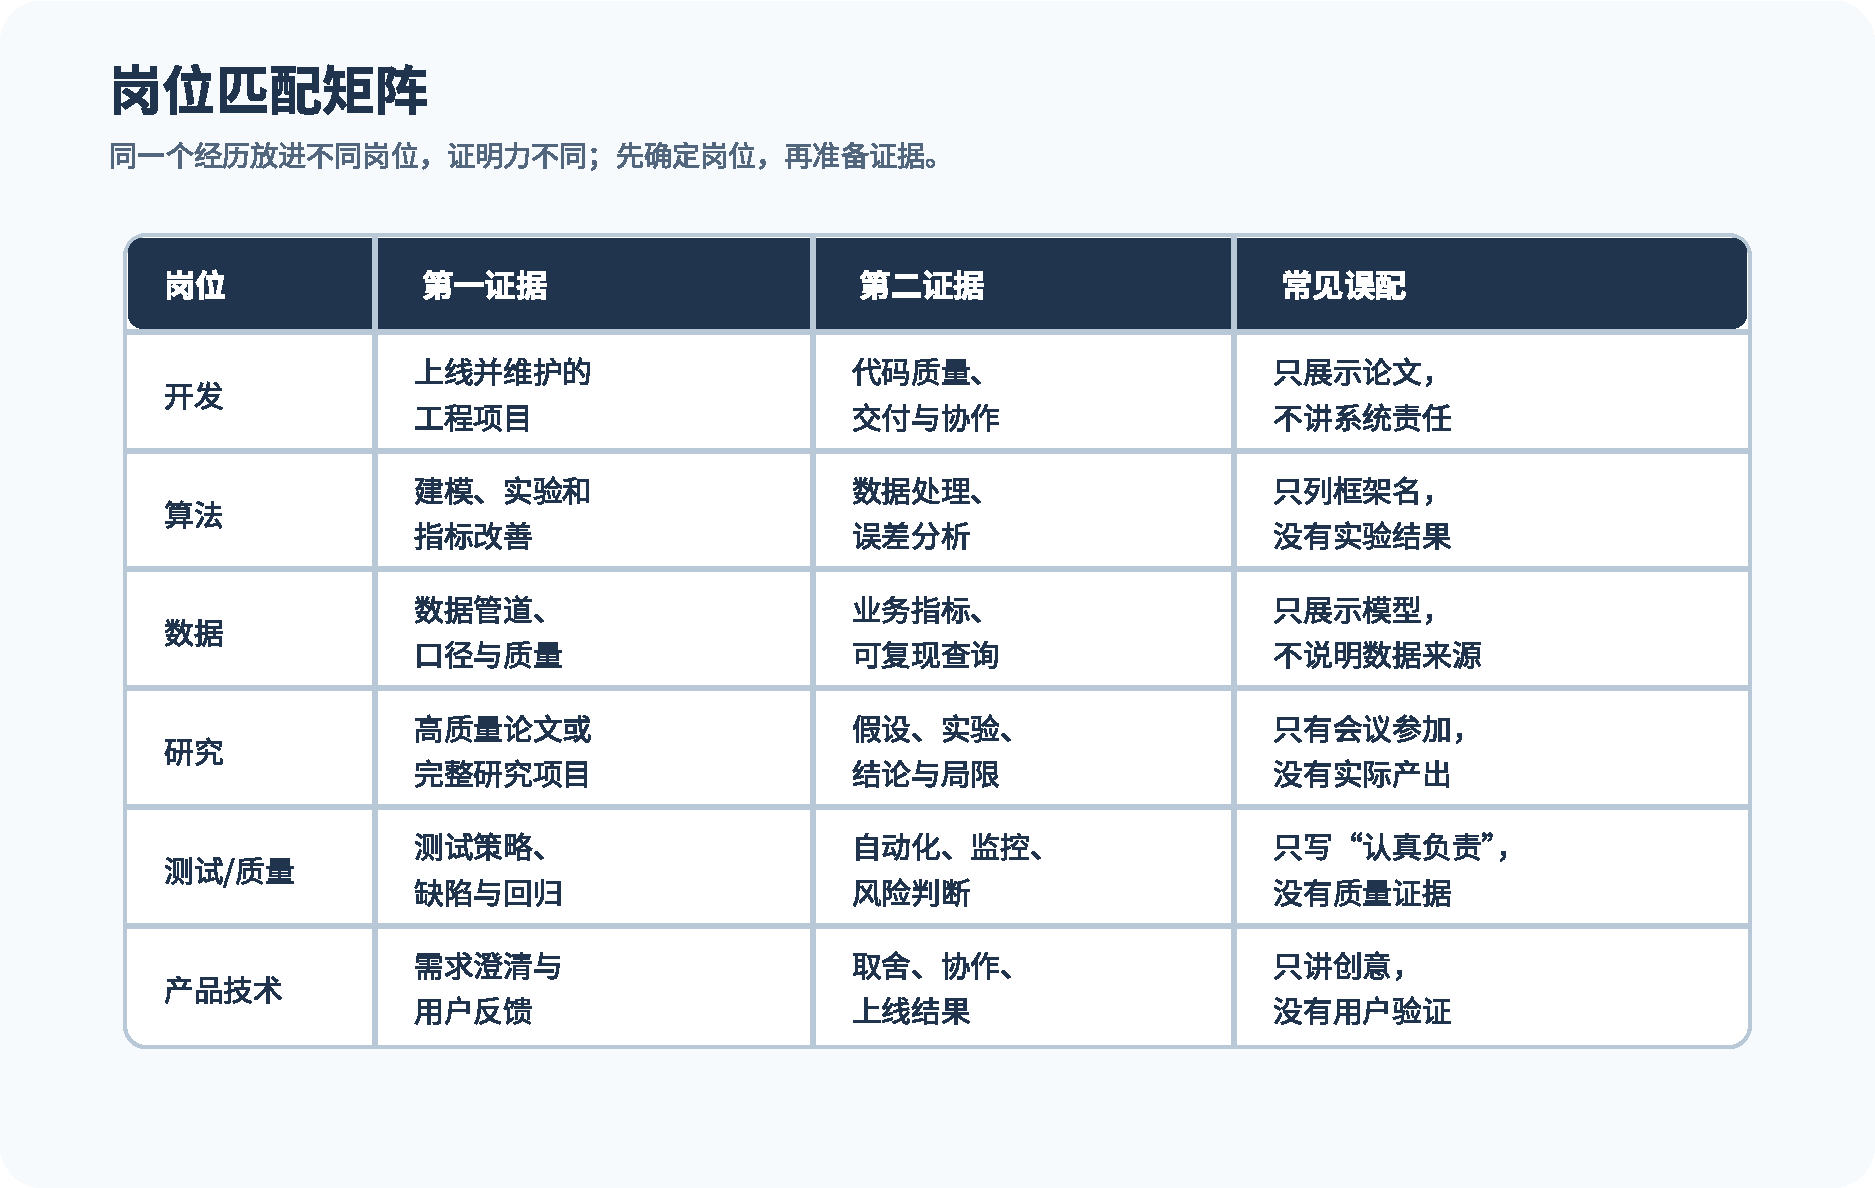
\includegraphics[width=1.0\textwidth]{assets/pdf/role_match_matrix.pdf}
\par\nopagebreak\smallskip
\captionof{figure}{同一段经历在不同岗位上的证明重点不同}
\end{center}
\section{2026 年，校招在变什么}
这一节没有预言，只讲已经能观察到的变化。

麦可思研究院《2026 年中国本科生就业报告》显示，2025 届本科生毕业半年后的平均月收入为 6435 元，计算机科学与技术、软件工程已跌出月收入前十；排在前面的换成了微电子科学与工程、电子科学与技术、自动化、光电信息科学与工程等硬科技专业\footnote{麦可思研究院《2026 年中国本科生就业报告》（2026 年 6 月）；本稿未获全文，数字本稿未见原始报告全文，转引自 TechWeb 2026 年 7 月 6 日报道，引用前请核对原报告。}。国家统计局的数据显示，2025 年 12 月全国城镇不包含在校生的 16--24 岁劳动力失业率为 16.5\%，已连续四个月下降\footnote{国家统计局 2025 年 12 月分年龄组失业率数据，2026 年 1 月 22 日发布。该口径不含在校生，衡量的是已进入劳动力市场的青年，不等于应届毕业生的就业率。}。

\textbf{第一，初级 CRUD 岗位在收缩。} 过去大量岗位做的是“把需求翻译成增删改查”，这部分正在被工具吃掉。企业更愿意招能处理系统边界、能定义问题的人，单纯会写接口的岗位变少了。

\textbf{第二，AI 相关岗位在增加，但门槛没有降低。} 算法岗依旧看论文和竞赛，AI 工程岗看的是推理优化、评测、数据管线、成本控制——这些都需要扎实的系统能力，不是调 API 能补上的。但要注意口径：猎聘大数据显示，2026 年 1--5 月机器学习岗位 1 年以下经验的需求同比下降 71.43\%，图像算法下降 66.67\%，软件测试下降 52.94\%\footnote{猎聘大数据，本稿未见原始报告全文，转引自 TechWeb 2026 年 7 月 6 日报道。}。总量在增、入门岗位在收缩，这是 2026 年校招最需要认清的走势。

\textbf{第三，面试在“防 AI”。} 面试官越来越常做的三件事：让你口述而不是粘贴、追问设计取舍、给一个改过的代码让你找 bug。背下来的答案在这些问题前失效得很快。

\needspace{5\baselineskip}
\captionof{table}{2026 年校招在变什么}
\begin{center}\small
\begin{tabularx}{\linewidth}{p{0.24\linewidth}p{0.30\linewidth}Y}
\toprule
变化 & 对学生的直接影响 & 现在就该补的 \\
\midrule
初级开发岗减少 & 简历上的“CRUD 项目”不再稀缺 & 一个能讲清故障与取舍的系统 \\
AI 工具普及 & Demo 门槛降低，深度变得值钱 & 评测、数据质量、成本意识 \\
招聘流程更长 & 池子与排序挂变多 & 心态与备选方案 \\
技术栈迭代快 & 学的框架可能毕业就换 & 计算机基础与调试能力 \\
\bottomrule
\end{tabularx}
\end{center}

一个可操作的判断：如果你做的项目，换一个熟练使用 AI 工具的人两周也能做出来，那它在面试里就不构成证据。真正稀缺的是“你解决过一个别人不愿意解决的麻烦”。


\clearpage\chapter{从分层市场到第一家公司}
\section{先说真话}
学历初筛是真实存在的。同一份简历，985 和双非被看到的概率不同，这不是阴谋，是筛选成本下的必然。承认这一点，才能谈策略；假装它不存在，只会让你在错误的战场上空耗。

供给端同样在放大：截至 2025 年 10 月，全国有 995 所高校开设计算机科学与技术专业；2024 年计算机类招生计划 43.5 万人，比 2023 年增加 4 万余人\footnote{阳光高考网统计数据（截至 2025 年 10 月 13 日），本稿未见原始报告全文，转引自 TechWeb 2026 年 7 月 6 日报道。}。这意味着“计算机＝稀缺”早已不成立，稀缺的只可能是具体的证据。

但“初筛不利”不等于“没有路径”。这一章讲的是：当你不在名单前列时，怎么把有限的证据用在正确的地方。

\section{三条路径}
\textbf{路径一：错位竞争。} 避开所有人都盯着的岗位（大厂算法、互联网后端），去那些缺人、且不那么看学校的领域：垂直行业的软件（医疗、工业、能源、物流）、嵌入式与硬件、测试开发、数据工程、政企信息化。这些地方的技术门槛不低，但竞争者少，你的项目更容易被看见。

\textbf{路径二：跳板。} 小厂或本地企业日常实习 → 中厂实习或校招 → 大厂社招。前两步不需要名校，需要的是“能把活干完”的证据。很多人卡在第一步，是因为只想一步到位。

\textbf{路径三：非标准入口。} 开源项目的持续贡献、外包与驻场、竞赛（不是水赛，是有真实工程量的比赛）、校内实验室的横向项目。这些入口不看学校，看产出。

\needspace{9\baselineskip}
\section{证据怎么组合才对冲学历}
\needspace{5\baselineskip}
\captionof{table}{不同处境下的证据组合}
\begin{center}\small
\begin{tabularx}{\linewidth}{p{0.22\linewidth}p{0.30\linewidth}Y}
\toprule
你的处境 & 最有效的证据 & 不要在什么地方浪费力气 \\
\midrule
双非、无实习 & 一个真实用户使用的系统 + 部署与维护记录 & 海投头部大厂算法岗 \\
双非、有日常实习 & 实习中的完整交付 + 量化结果 & 反复改简历格式 \\
普通院校、项目强 & 可复现的作品 + 技术博客 & 参加含金量低的比赛凑数 \\
资源有限（无设备、需兼职） & 小而完整、可讲清取舍的项目 & 追大模型全流程训练 \\
跨专业 & 补课记录 + 一个证明迁移能力的项目 & 解释“我为什么转专业” \\
\bottomrule
\end{tabularx}
\end{center}

\section{一个反直觉的建议}
如果你现在大二、双非、没有资源，最不该做的是“同时准备考研、实习、竞赛、开源”。你最该做的是选一条路径，把它走到能被验证的程度——比如用八个月做一个真正有人用的系统，然后带着它去投递。

分散的努力看起来安全，实际上让你在每个战场上都不够强。分层市场里，弱者的优势从来不是“全面”，而是“在某个具体问题上比名校生更深”。

\section{关于“要不要考研翻身”}
这是一个真实存在的选项，但它不是万能钥匙。判断标准是：你想去的岗位，招聘要求里写的是不是硕士？如果写的是“本科及以上”，读研的边际收益可能不如三年工作经验；如果写的是“硕士及以上”，那就是硬门槛。

不要为了“证明自己”去考研，要为了“跨过某道具体的门槛”去考研。前者容易消耗三年，后者至少有一个可验证的目标。


\section{选择第一家公司}
\subsection{公司选择是资源约束下的决策}
大厂、中型公司、初创公司和研究机构不是简单的高低排序，而是训练密度、稳定性、自由度、资源、信用和风险的不同组合。你应该先写自己的约束：需要多高的收入，能承受多少不确定性，是否需要城市稳定，是否有家庭责任，想积累什么能力。

\begin{toolbox}
\needspace{5\baselineskip}
\captionof{table}{Offer 权重表}
\begin{center}\footnotesize
\begin{tabularx}{0.94\linewidth}{p{0.22\linewidth}p{0.10\linewidth}p{0.10\linewidth}p{0.10\linewidth}p{0.10\linewidth}}
\toprule
指标 & 权重 & 公司 A & 公司 B & 公司 C \\
\midrule
学习与训练密度 & & & & \\
岗位匹配度 & & & & \\
团队与直属负责人 & & & & \\
收入与稳定性 & & & & \\
可带走的能力与成果 & & & & \\
工作时间与健康成本 & & & & \\
城市与家庭约束 & & & & \\
\bottomrule
\end{tabularx}
\end{center}
\end{toolbox}

\subsection{初创公司的六个问题}
选择初创公司，本质上是在选择一群人、一个问题和一段高不确定性的时间。至少要问：
\begin{enumerate}
\item 创始人与方向是否匹配？
\item 创始人是否真正做过从零到一的定义、验证和整合？
\item 公司解决的是真实需求，还是技术自嗨？
\item 团队是否低 ego、能快速迭代并承认错误？
\item 在融资环境变化时，公司能否继续活下去？
\item 这家公司是否值得你投入这段时间？
\end{enumerate}

这六个问题只能作为尽调入口，不能替代合同和财务核查。还应确认薪酬、发放时间、社保、公积金、试用期、加班、股权、知识产权、汇报关系和项目优先级。

\subsection{技术光环不等于创业能力}
技术光环和能力是两件事。大厂履历、技术分享会上的表达能力、一次漂亮的融资，都不能证明一个人能脱离平台资源定义问题、拿到第一批用户并持续交付。判断一家初创公司时，与其看创始人讲得多好，不如看他有没有过“从零把一件事做成、并且靠它活下来”的记录，以及团队在融资环境变冷时还剩多少时间。

\begin{center}\vspace*{0pt}
\includegraphics[width=1.0\textwidth]{assets/pdf/offer_decision_tree.pdf}
\par\nopagebreak\smallskip
\captionof{figure}{先看硬约束，再比较成长资本与生活成本}
\end{center}
\subsection{offer 里的钱怎么算}
第一份 offer 的谈判空间通常很小，但“看懂”是必须的。

先建立一个数量级：TTC 对 AI 人才样本的统计显示，年薪中位数约 50 万元，前 10\% 的门槛超过中位数的两倍（120 万元以上）；25 分位到中位数差 15 万，中位数到 75 分位差 30 万。要注意这是有工作经验的 AI 人才样本，不是应届校招数字——用它校准“这个行业的天花板在哪”可以，用它对标第一份 offer 会失真。\footnote{TTC AI 人才研究院《AI 人才市场图谱》，2026 年，第 19 页“薪资整体分布区间”。}

\needspace{5\baselineskip}
\captionof{table}{offer 里的钱：要问清的事与常见坑}
\begin{center}\small
\begin{tabularx}{\linewidth}{p{0.20\linewidth}p{0.30\linewidth}Y}
\toprule
项目 & 要问清楚的事 & 常见坑 \\
\midrule
月薪与月数 & base 多少、发几个月、是否有 13/14 薪 & 用最高月数宣传，实际按最低发 \\
绩效与年终 & 占比多少、按什么考核、什么时候发 & 年终奖写在 offer 里但附条件 \\
股票／期权 & 授予数量、行权价、四年归属节奏 & 把未上市期权按面值算进总包 \\
签字费 & 是否一次性、是否需服务满一年 & 提前离职要退还 \\
公积金与社保 & 缴纳基数与比例 & 按最低基数缴，总包缩水 \\
试用期 & 时长、薪资比例、转正标准 & 试用期工资打八折且无明确标准 \\
\bottomrule
\end{tabularx}
\end{center}

判断一个 offer 不能只看总包数字，要看“确定能拿到的部分”和“看条件才拿到的部分”各是多少。把确定的年现金收入单独算出来，再比较。

\subsection{三方协议：三个必须问的问题}
\begin{enumerate}
\item \textbf{违约金多少、什么情况下触发？} 一般是几千到一个月工资，但有的公司写得很高。
\item \textbf{毁约流程是什么？} 拿到更好的 offer 想毁约，需要原公司出解约函，流程要走多久。
\item \textbf{档案和户口怎么转？} 2023 年起就业报到证已不再发放，档案转递与户口迁移按学校和人社部门的流程办理；不同城市要求不同，以当年的通知为准。\footnote{国务院办公厅《关于进一步做好高校毕业生等青年就业创业工作的通知》（国办发〔2022〕13 号）：取消就业报到证，2023 届起不再发放。全文见中国政府网。}
\end{enumerate}

遇到“今天不签就没了”这类话术，处理办法见第 13.4.3 节：先问能不能给到明天中午，再做决定。

\subsection{竞业与保密}
应届生很少注意这一块。入职合同里如果有竞业限制条款，要确认三件事：范围有多大、期限多长、补偿怎么算。按法律规定，竞业限制期间公司需要按月支付经济补偿\footnote{最高人民法院《关于审理劳动争议案件适用法律问题的解释（一）》第三十六至三十八条。}；如果约定了竞业限制却没有约定补偿，劳动者履行义务后可以要求按法定标准支付，不能简单理解成“条款自动无效”。

保密协议同理：它约束的是你带走公司数据与商业秘密，不约束你带走自己的能力。写简历时，能写“我做了什么、解决了什么问题”，不能写客户名单、内部数据、未公开方案。


\clearpage\chapter{从实习到入职：第一份工作的前半年}
实习不是上课。学校的项目里，你是唯一的决策者；实习里，你是链条上的一环。这一章讲的三件事，决定了你能不能把两个月过成一段能写进简历的经历。

\section{第一件事：主动对齐，而不是等人来教}
mentor 通常带两三个实习生，还要开自己的会。你不主动，他就默认你没问题——直到交付前一天发现方向错了。

一个可用的节奏：

\begin{itemize}
\item \textbf{接任务时}：用自己的话复述一遍需求与验收标准，问一句“我理解得对吗”。
\item \textbf{每天}：一句话同步进展和卡点（可以发在群里），不要等到周五。
\item \textbf{卡住超过半天}：先说“我卡在哪、试过什么、需要什么帮助”，再继续试。
\item \textbf{每周}：写一份三行的周报——做了什么、结果如何、下周计划。
\end{itemize}

这些动作看起来很笨，但它们构成了“可被信任”的证据。实习结束时，mentor 愿意给你写推荐语，靠的就是这些。

\section{第二件事：把边缘任务做成可迁移的证据}
大概率你拿到的第一件事是：修几个 bug、写个内部脚本、整理数据、补文档。这不是刁难，是新人的常态。

关键是怎么处理它：

\needspace{5\baselineskip}
\captionof{table}{边缘任务的两种做法}
\begin{center}\small
\begin{tabularx}{\linewidth}{p{0.24\linewidth}p{0.32\linewidth}Y}
\toprule
拿到的任务 & 平庸做法 & 可以写进简历的做法 \\
\midrule
修 bug & 改完提测，不说话 & 定位根因、补一条回归测试、记录同类问题 \\
写内部脚本 & 能跑就行 & 加上参数校验、日志、失败重试，交给别人也能用 \\
整理数据 & 手工处理一遍 & 做成可复用的清洗流程，说明数据质量问题的来源 \\
补文档 & 照着代码抄 & 画出调用链，标出容易踩坑的边界 \\
\bottomrule
\end{tabularx}
\end{center}

差别不在任务大小，而在你有没有把“一次交付”变成“可复用的东西”。三个月里做成两件这样的事，比做二十个边角需求更有价值。

\section{第三件事：提前确认有没有转正名额}
不要等到实习快结束才问。合适的时点是实习满一个月、你已经开始独立承担任务之后，问 mentor：

“我想知道团队今年的转正名额大概是什么情况，以及我需要在哪些方面达到什么标准，才比较有机会？”

这句话不冒犯，反而显得你在认真规划。大多数 mentor 会给出真实信息：有没有名额、看什么、什么时候评估。知道了，你才知道该把力气放在哪。

\section{转正答辩怎么讲}
多数公司的转正答辩是 10--15 分钟。结构比内容重要：

\begin{enumerate}
\item 背景：我接手的任务是什么，为什么要做。
\item 我做了什么：职责边界、关键决策、遇到的困难。
\item 结果：指标、影响范围、被谁使用。
\item 反思：如果重做会怎么改，还有哪些没做完。
\item 下一步：如果留下，我打算接手什么。
\end{enumerate}

不要把它讲成流水账。面试官想听的是“这个人能不能独立负责一件事”。

\section{三条红线}
\begin{itemize}
\item 不要为了跑通而绕过权限、跳过校验、动生产数据。一次图方便，可能毁掉整段实习。
\item 不要藏问题。出了问题第一时间说，比事后被发现代价小得多。
\item 不要消失。请假、离职、回学校，都要提前说清楚，交接文档写好。
\end{itemize}

\section{离开前要带走的东西}
实习结束时，带走四样东西：一份交接文档（别人能照着接手）、一份成果清单（做了什么、结果如何、可复现的证据在哪）、一段可用的评价（问 mentor 愿不愿意做你的推荐人）、一份复盘（哪些判断错了、下次怎么改）。

前两样决定你能不能在简历和面试里讲清楚这段经历，后两样决定你下一次能不能做得更好。很多人在实习结束那天只发了一句“谢谢”，把最值钱的东西留在了公司里。


\section{入职后的第一份工作}
\subsection{前九十天先建立可靠性}
入职前九十天不是证明自己什么都会，而是建立可被团队信任的工作方式：理解目标、确认边界、记录假设、及时同步风险、让别人能够接手。

\begin{enumerate}
\item 前 30 天：理解业务、系统、权限、数据和团队协作方式。
\item 31--60 天：独立承担一个边界清楚的任务，补齐测试、日志和文档。
\item 61--90 天：交付一个可复盘的结果，说明指标、失败和下一步。
\end{enumerate}

带走能力，不带走秘密。可迁移资本包括能力、方法、公开作品、问题理解、人脉和信用。公司代码、内部数据、客户资料、未公开方案和商业秘密不属于个人作品集。写简历时要能清楚区分：我做了什么、团队完成了什么、平台提供了什么。

\begin{center}\vspace*{0pt}
\includegraphics[width=1.0\textwidth]{assets/pdf/onboarding_90_days.pdf}
\par\nopagebreak\smallskip
\captionof{figure}{入职 90 天的理解、交付、反馈与复盘循环}
\end{center}

\chapter{钱、家庭、身体与心态}
\section{不是所有人都拥有同样的试错预算}
“年轻就应该大胆试错”只在一定条件下成立。城市成本、家庭责任、健康、签证、照护、债务和心理状态都会改变一个人的可承受风险。把这些写进决策表不是不够勇敢，而是把现实纳入模型。

可以先看一个行业基数：2024 年城镇非私营单位中，信息传输、软件和信息技术服务业就业人员年平均工资 238966 元，是全国城镇非私营单位平均（124110 元）的 1.9 倍\footnote{国家统计局：2024 年城镇非私营单位就业人员年平均工资 124110 元，其中信息传输、软件和信息技术服务业 238966 元；城镇私营单位 69476 元（2025 年 5 月 16 日发布）。}。同年全国城镇私营单位平均为 69476 元，行业内私营企业的平均工资低于非私营，但岗位之间的差异远大于这个平均数。数字只说明行业整体所处的位置，不说明某个人的起薪。

\section{用现金流看待选择}
学生可以先计算最低生活成本、可用储蓄、家里能够提供的支持、工作空窗期和最坏情况下的回退方案。选择创业、低薪实习或异地工作前，至少回答：如果三个月没有收入，我怎么生活；如果项目失败，我能回到哪条路径；这次选择是否会损害学业、健康或家庭安全。

工作时间也是价格。岗位比较不能只看月薪。通勤、加班、睡眠损失、社交成本和恢复时间都会改变真实收益。一个看起来多出的收入，如果让你失去基础健康和长期学习能力，可能不是更高的回报。

把身体写进 offer 表。工作时间与健康成本不应该是附加项。建议记录睡眠、久坐、饮食、运动和情绪恢复的最低条件。持续的身体问题需要专业医疗帮助，职业规划不能替代诊疗。

\section{心态：焦虑、同伴压力与重新开始}
\subsection{先承认一件事}
前面所有章节都默认你能按计划执行。但真实情况往往是：投了五十份简历没有回音，室友已经拿到大厂 offer，项目卡了三天没人可问，你打开电脑只想刷手机。

这不是意志力问题。人在持续的负反馈里，行动能力本来就会下降。这一章讲的是：在这种状态下，怎么让自己重新动起来。

\subsection{同伴压力：把“比较”换成“基线”}
看到别人拿到 offer 就慌，是因为你在拿自己的“现在”比别人的“结果”，而你不知道别人的起点、路径和运气。

一个更可用的做法是建立自己的基线：只和自己三个月前比。三个指标就够了——能独立完成的项目规模、能过几道中等题、简历上能写出几条经得起追问的经历。基线在涨，就是在进步。

\subsection{冒充者综合征：把“我不行”拆成可验证的话}
“我不行”是一句无法验证的话，所以它永远不会被推翻。把它改写成具体陈述：

“我讲不清项目的并发处理” → 可以补。
“我笔试过不了” → 可以刷题。
“我没有实习” → 可以在两周内投二十家日常实习。

一句可验证的陈述，对应一个可以执行的动作。情绪不需要被消灭，只需要被翻译。

\subsection{最小启动：五分钟规则}
状态最差的时候，不要定“今天学四小时”这种目标，它只会带来又一次失败。改用五分钟规则：打开项目，只做五分钟，做完就可以停。

大多数时候，五分钟之后你会继续做下去——启动的阻力远大于持续的阻力。这个方法不解决所有问题，但能解决“完全启动不了”的那一类。

\subsection{什么时候该停下来}
如果出现持续两周以上的失眠、食欲变化、无法集中、对什么都提不起兴趣，或者身体出现明显症状（心悸、胃痛、持续头痛），这不是“再努力一点”能解决的。去看医生，或者找学校的心理咨询中心。

职业规划不能替代诊疗。把身体和情绪当成系统的一部分来维护，和刷题、做项目一样，是长期竞争力的一部分。

\subsection{一个可以今晚就做的动作}
写下三件事：
\begin{enumerate}
\item 我现在最焦虑的一件具体的事（不是“我的未来”，而是“下周三的面试”）。
\item 这件事里我能控制的部分（准备三个问题、练一遍自我介绍）。
\item 今晚就能做的、不超过二十分钟的一步。
\end{enumerate}

把注意力从“无法控制的整体”移到“可以控制的一步”，是缓解焦虑最朴素也最有效的方式。


\chapter{信息与规则：别被数字牵着走}
\section{一张图不等于一个结论}
薪资分位数、人才年龄、城市集中度和岗位数量都需要样本、口径、时间、行业范围和统计方式。没有这些信息，数字只能帮助你产生问题，不能直接告诉你应该选择哪条路。

读数据之前，先练基本功：查官网原文而不是二手转述，核对发布日期而不是凭印象，对任何“据说”留一个问号。信息素养不是聪明，是一套习惯——同一份政策，官网原文和群里转发的截图，往往是两件事。\footnote{《上海交通大学学生生存手册》“认识信息素养”列出了查证、辨伪、隐私与提问的具体做法。\url{https://github.com/1638410/SurviveSJTUManual/blob/master/li-zhi-pian/ren-shi-xin-xi-su-yang.md}。}

\section{报告的四层阅读法}
第一层看发布者和利益关系；第二层看样本和定义；第三层看数字如何计算；第四层问它能否指导自己的决策。报告说“某类人才集中在几个城市”，不代表你必须去这些城市；报告说“某经验稀缺”，也不代表你只要拥有标签就能获得溢价。

\begin{toolbox}
\needspace{5\baselineskip}
\captionof{table}{数据来源卡}
\begin{center}\small
\begin{tabularx}{0.92\linewidth}{p{0.18\linewidth}YYY}
\toprule
项目 & 记录 & 核查问题 & 结论边界 \\
\midrule
发布者 & & 谁资助或发布？ & \\
时间 & & 是否已经过时？ & \\
样本 & & 代表谁，不代表谁？ & \\
指标 & & 分母和口径是什么？ & \\
用途 & & 能支持哪一个决定？ & \\
\bottomrule
\end{tabularx}
\end{center}
\end{toolbox}

\section{从数据回到个人行动}
数据最有价值的用途是帮助你决定下一次调查什么、做什么实验和向谁提问。例如，发现某岗位竞争激烈，不应立即得出“我没机会”，而可以拆成：岗位需要哪些证据，我缺哪项证据，证据能否在八周内补齐，是否存在相邻岗位。

\section{组织里的程序公平：求职者视角}
\subsection{你会遇到的几种不公平}
求职不是一场完全公平的考试。你可能遇到：简历因为学校被筛掉、面试安排临时取消、流程走到一半岗位冻结、口头承诺的薪资入职后打折、试用期没有明确标准就被判定不合格。

这些事不都是恶意，有的是流程混乱，有的是信息不对称，有的是行业周期。但对个人来说，结果是一样的：你的时间和机会被消耗了。

这一章讲两件事：怎么提前识别一家公司是否尊重程序；当你从求职者变成筛选者时，怎么不重复你讨厌的做法。

\needspace{9\baselineskip}
\subsection{识别信号：一家公司是否尊重程序}
\needspace{5\baselineskip}
\captionof{table}{判断公司是否尊重程序的两个信号}
\begin{center}\small
\begin{tabularx}{\linewidth}{p{0.24\linewidth}p{0.30\linewidth}Y}
\toprule
观察点 & 好信号 & 坏信号 \\
\midrule
面试流程 & 提前告知几轮、多长时间 & 临时加面、不说明下一轮时间 \\
反馈 & 明确告知结果，哪怕拒绝 & 一直“等通知”，再无回复 \\
offer & 书面、条款清晰、给考虑时间 & 口头承诺、催当天签、条款含糊 \\
试用期 & 有明确考核标准 & “看表现”，没有书面标准 \\
加班 & 提前说明节奏与补偿 & 避而不谈，只说“弹性” \\
离职 & 有交接流程、按合同执行 & 卡档案、拖离职证明 \\
\bottomrule
\end{tabularx}
\end{center}

单个坏信号不一定说明问题，但如果几条同时出现，就值得提高警惕。尤其注意“催签”和“口头承诺”这两项——它们往往意味着对方知道条件经不起比较。

\subsection{遇到逼签怎么办}
“今天不签就作废”是常见话术。可以这样回应：

“我很希望加入，但三方涉及违约金和档案，我需要一天时间确认条款。明天中午前我一定给明确答复。”

大多数情况下，对方会给这一天。如果给不了，这本身就是一个信息。真正缺人的团队，不会因为一天而撤掉一个合适的人。

\subsection{被不公平对待之后}
一次拒绝不能说明你的能力，也不一定能说明公司的好坏——招聘是排序，不是评分。但如果你记录下每次的流程节点（投递日期、笔试、面试轮次、反馈方式），走完十家之后，你会看到一些模式：哪类公司回得快、哪类公司总是无疾而终、你的简历在哪一类公司会卡住。

这些记录不解决情绪，但能让你下一次把力气用在更可能的地方。

\subsection{承认结构，但不放弃行动}
教育资源、家庭经济、地区、信息渠道和运气，都会影响一个人能不能被看见。承认这些差异，不会削弱努力的价值；否认它们，反而会让建议变得空洞。

同样，技术乐观也需要边界。谈 AI 时除了问“它能做什么”，也可以问：谁得到收益，谁承担风险，哪些错误会由普通用户承受。一个不包含责任边界的技术方案，只是一次功能展示。


\chapter{复盘与结语：把一年变成一个可复盘的系统}
\section{年度不是愿望清单}
一年计划不应该堆满目标，而应该有一条主线、两到三个支持动作和明确的停止条件。主线是当前最重要的能力或问题；支持动作是基础维护、人脉、健康和财务；停止条件用于防止计划变成无法退出的负担。

每季度问五个问题：\begin{enumerate}
\item 我真正交付了什么，而不只是学习了什么？
\item 哪项能力获得了外部反馈？
\item 哪个判断被证据推翻？
\item 哪个代价超过了我预期？
\item 下一季度要继续、暂停、转向还是彻底放弃什么？
\end{enumerate}

不要把身份当成合同。“我是 AI 人”“我是竞赛选手”“我一定要创业”都可以在某个阶段提供动力，但它们不是不可更改的身份合同。身份应该帮助你组织行动，而不是阻止你承认新的证据。

成功与失败都能提取资产。成功要问哪些条件可以复制，哪些只是运气；失败要问哪些机制需要改进，哪些结果只是不可控。把所有结果都归因于自己，会产生虚假的自责或自信；把所有结果都归因于环境，则会失去行动能力。
\clearpage\section{一份年度复盘的模板}
\begin{toolbox}
\needspace{5\baselineskip}
\captionof{table}{年度复盘卡}
\begin{center}\small
\begin{tabularx}{0.92\linewidth}{p{0.24\linewidth}YY}
\toprule
维度 & 今年的事实 & 明年要改的一件事 \\
\midrule
交付了什么 & & \\
哪项能力有外部反馈 & & \\
哪个判断被推翻 & & \\
付出了什么代价 & & \\
关系与帮助 & & \\
健康与状态 & & \\
\bottomrule
\end{tabularx}
\end{center}
\end{toolbox}

写的时候只写事实，不写评价。“今年投了 40 家、面了 6 家、拿到 1 个 offer”是事实，“今年很失败”是评价。事实能指导下一步，评价只会加重情绪。


\clearpage\section{练习：三分钟与十分钟版本}
给每段重要经历准备两个版本，写在卡片上，面试前过一遍。

\begin{toolbox}
\textbf{三分钟版}：背景一两句、我的责任、关键动作、结果、一句复盘。\\[2pt]
\textbf{十分钟版}：在三分钟版基础上，补上设计取舍、失败过的方案、协作与冲突、数据口径、边界与下一步。

\smallskip
用手机给自己录音，回放时只听三件事：有没有说清楚“我做了什么”、有没有具体数字、有没有超过时限。
\end{toolbox}


\section{结语：从礼堂到秋招不是终点}
你不可能在入学典礼那天知道秋招现场的所有问题，也不可能在拿到第一份 offer 时知道十年后的答案。

你能做的是让每一次选择都留下更多信息：你试过什么，做成了什么，哪里失败，谁给过帮助，什么约束影响了结果，下一次应该怎样调整。

技术会变，岗位会变，公司会变，个人也会变。真正可迁移的不是某个永远热门的关键词，而是理解问题、建立证据、与人合作、承担责任和重新学习的能力。

你可以追求收入、稳定、技术深度、社会意义、自由时间或志同道合的人。不要假装这些目标永远一致。成熟的选择不是找到没有代价的道路，而是看清自己愿意承担什么代价，并在条件变化时有能力重新选择。

\subsection*{致谢}
这本书里最有用的一些判断，不是我一个人想出来的。带我们入门深度学习的学长，愿意在我什么都不懂的时候回消息的中科院博士网友，实习时把我当同事而不是实习生用的领导，还有在我拿不准边界时替我解释过规则的法务与律师——他们各自补上了我当时的盲区。

把这本书写出来，也是想把这种“有人愿意花十分钟回答一个笨问题”的运气，尽量传下去。

\appendix
\chapter{四类读者的行动路线}
\begin{longtable}{p{0.14\textwidth}p{0.24\textwidth}p{0.26\textwidth}p{0.20\textwidth}}
\toprule
阶段 & 先解决的问题 & 90 天行动 & 形成的证据 \\
\midrule
\endhead
高中 & 了解专业和岗位，避免只看名词 & 访谈 3 人；体验 2 个小项目；阅读 3 份课程方案 & 方向假设、问题清单 \\
大一 & 建立基础，获得反馈 & 完成一门基础课；参加一次团队项目；找到一位可请教的人 & 学习记录、项目卡 \\
大二至大三 & 选择岗位族并收敛 & 做一份 8--12 周代表作；拆解 20 份 JD；争取一次真实交付 & README、实验、反馈、复盘 \\
大四 & 把经历匹配到机会 & 完成岗位矩阵、简历、模拟面试和 offer 权重表 & 可验证简历、面试记录、决策表 \\
\bottomrule
\end{longtable}

\chapter{冷启动通信脚本库}
这一章是可以直接改着用的模板。B.1 给了正反两个版本作示范，其余各条是推荐版本——写法逻辑相同：说明你是谁、说清你要什么、降低对方的成本。

\section{给陌生校友或行业前辈的第一条消息}
\begin{casebox}
\textbf{反例：}“学长你好，我是 XX 学校的学生，能不能加个微信，想向你请教一下职业规划。”
\end{casebox}

问题：没有具体问题，成本全在对方身上。

\begin{casebox}
\textbf{推荐：}“X 学长你好，我是 XX 大学计算机学院大三的学生，正在准备后端方向的实习。看到你在 XX 公司的 XX 团队做过订单系统，我最近在做一个校园二手交易平台，遇到了分库分表后订单查询变慢的问题（现在 P95 约 800ms）。想请教一个问题：你们当时是按用户 ID 还是按时间分片的？如果不方便，能推荐一篇你们参考过的文章也可以。谢谢！”
\end{casebox}

三个要点：说清身份、给出一个具体且窄的问题、允许对方低成本地回答。

\section{大一没有基础，怎么联系本校实验室}
\begin{casebox}
\textbf{推荐：}“X 老师您好，我是计算机学院大一学生 XXX，学号 XXX。我读了您组里 2025 年那篇关于 XX 的论文，对第三部分的实验设计很感兴趣。我目前学完了 C 语言和数据结构，能写 Python 脚本。想请问组里是否接收大一的本科生做一些基础工作，比如数据整理、复现实验或工程支持？如果不方便，能否推荐我该先补哪门课？”
\end{casebox}

关键：证明你读过他的东西、说明你会什么、把要的东西缩小到“基础工作”。

\section{请人内推}
\begin{casebox}
\textbf{推荐：}“X 哥你好，看到你们组在招 XX 岗（JD 链接），我投了简历但还没消息。我的情况：XX 学校 XX 专业，有一段 XX 公司的日常实习，做过 XX 系统（GitHub 链接），和这个岗位的 XX 要求比较匹配。如果方便，能否帮我内推？简历在附件，如果不合适也没关系，谢谢你。”
\end{casebox}

内推不代表要对方为你背书，只需要他花 30 秒点一下。所以要给足信息、不要给压力。

\section{队友摆烂，怎么开口}
\begin{casebox}
\textbf{推荐：}“这周的分工里，登录模块还差接口和测试。我想确认一下你的时间：如果这周确实排不开，我们可以把它拆小，或者换给另一个人；如果继续由你负责，能不能定在周五晚上给一个能跑通的最小版本？我需要提前知道，不然下周的联调会卡住。”
\end{casebox}

公式：陈述事实（不是评价人）+ 给出选项 + 明确时间。

\section{自己想退出项目}
\begin{casebox}
\textbf{推荐：}“我这学期在准备实习，能投入项目的时间从每周 10 小时降到 3 小时左右。为了避免拖累进度，我想把手上负责的 XX 模块整理成文档和可运行的代码交接出去，预计本周日完成。如果需要，我可以再带一个人一周。很抱歉给团队添麻烦。”
\end{casebox}

体面退出的三个动作：提前说、交出可用的东西、给出过渡期。

\section{跟 HR 谈 offer 延期}
\begin{casebox}
\textbf{推荐：}“X 老师您好，非常感谢团队的认可。我目前还有另一家公司的流程在走，预计下周三有结果。想请问 offer 的答复期限能否延长到下周五？无论结果如何，我都会在周五前给出明确答复。”
\end{casebox}

要点：给出明确的新期限、承诺会答复、不透露谁家的 offer。

\section{向 mentor 要反馈}
\begin{casebox}
\textbf{推荐：}“这两周我主要在做 XX，想请你抽 10 分钟给我一点反馈：一是我在需求理解上有没有偏差；二是我交付的东西质量够不够；三是我下个月可以在哪一块多承担一点。你直接说问题就好。”
\end{casebox}

大多数 mentor 不是不愿意给反馈，而是不知道你想听什么。给出三个具体维度，会得到真实得多的回答。

\section{跟父母谈职业选择}
\begin{casebox}
\textbf{推荐：}“我知道你们担心的是稳定和安全。我现在的计划是：先投暑期实习（2--4 月），如果拿到就去，同时准备考研作为备选；暑假结束前，我会根据结果决定走哪条路。这个安排里有哪些是你们最担心的，我们可以先把它列出来，一起查资料。”
\end{casebox}

父母反对往往不是反对你，而是反对“没有计划的冒险”。把计划、时间点和回退方案讲清楚，比反复争论“我喜欢什么”有效。


\chapter{项目卡与成果账本}
\begin{toolbox}
项目名称：\fillrule

问题与用户：\fillrule

我负责的边界：\fillrule

基线与指标：\fillrule

关键实验：\fillrule

失败与放弃的方案：\fillrule

结果与验证方式：\fillrule

别人可以复现或检查什么：\fillrule

下一步：\fillrule
\end{toolbox}

填写时注意三件事。第一，边界要写“不做什么”，面试官更关心你是否清楚范围。第二，指标要写清口径：多少人用、覆盖多少条数据、P95 还是平均。第三，可复现那一栏不能空着——仓库、部署地址、测试方法，至少留一样，否则这张卡在面试里就只是自述。

\section{成果账本与简历核查}
用这张表把你的经历翻译成岗位语言。填的时候注意三件事：责任要写到“我具体做了什么”，结果要能说清口径，边界要提前想好——面试官一定会问“这部分是你做的还是团队做的”。

\begin{toolbox}
\textbf{简历核查五问}\par\smallskip
\begin{enumerate}
\item 这一条里的数字，我能说出它怎么统计出来的吗？
\item 如果面试官追问三层，我还能答上来吗？
\item 这条经历对应目标岗位的哪一项要求？
\item 我说的是“我做的”，还是“我们做的”？
\item 这条能不能删掉而不影响岗位匹配？
\end{enumerate}
\end{toolbox}


\begin{longtable}{p{0.16\textwidth}p{0.24\textwidth}p{0.22\textwidth}p{0.20\textwidth}}
\toprule
经历 & 我的具体责任 & 结果证据 & 面试时的边界 \\
\midrule
\endhead
课程项目 & & & \\
竞赛 & & & \\
实习 & & & \\
开源 & & & \\
研究或论文 & & & \\
其他交付 & & & \\
\bottomrule
\end{longtable}

\chapter{术语表}
\begin{description}
\item[有限理性] 在信息、时间和计算能力有限的情况下做出可接受决策；它解释为什么职业规划需要持续更新。
\item[贝叶斯更新] 把新证据用于调整原有判断的比喻；本书不把它当作精确预测工具。
\item[真实期权] 保留未来选择的价值；探索越久也会有放弃深度积累的成本。
\item[护城河] 在具体问题上形成的较难替代的能力、作品、责任或关系资产。
\item[信号] 能让他人判断能力的可观察证据；信号强弱取决于真实性、相关性和可验证性。
\item[最小实验] 用有限时间和资源验证最危险假设的行动。
\item[代表作] 能清楚说明问题、责任、结果、边界和复现方式的项目或交付。
\item[系统可靠性] 对异常、超时、权限、日志、维护、交接和恢复的综合考虑。
\item[心理契约] 合作双方对彼此承诺、回报和公平的非正式期待；不等同于法律合同。
\item[程序公平] 让标准、流程、反馈和申诉机会能够被理解并一致适用。
\item[人岗匹配] 个人能力、兴趣、约束与岗位任务、环境和回报的组合关系。
\item[机会工程] 通过主动寻找信息、导师、项目和反馈，提高遇到机会的概率。
\item[冷启动] 在没有现成人脉与作品的情况下，用具体、低成本的请求建立第一次联系；关键是把对方的时间成本降到最低。
\item[证据五层] 把一段经历拆成存在、责任、交付、效果、迁移五个层次；低层证据不能写成高层结论。
\item[目标企业库] 二十到四十家长期跟踪的目标公司名单，按发现渠道、业务、匹配点与待核实问题维护。
\item[分层市场] 把雇主按学历门槛、面试风格、收入与流动性分成不同层级；同一份证据在不同层级的价值不同。
\item[转正实习] 暑期实习结束前的评估环节，通过即提前获得正式 offer；多数大厂的核心名额来源于此。
\item[企业地图] 从资本、信用、政策、学术、市场、技术、人才和雇主等第三方筛选结果出发建立的目标企业名单，用于长期跟踪和定向投递。
\item[定向投递] 先交叉验证企业信息和岗位匹配度、再针对性投递的做法；与按岗位名批量海投相对。
\end{description}



\chapter{主题索引}
本索引按主题列出主要讨论所在的章或节，便于跳读；标“章”的是整章讨论，标“节”的是具体段落。

{\small\begin{longtable}{p{0.30\linewidth}p{0.64\linewidth}}
\toprule
主题 & 位置（章 / 节） \\
\midrule
专业选择 & 第 1.4 节、第 7.1 节 \\
培养方案 & 第 1.4 节 \\
时间轴 & 第 2.1–2.2 节 \\
分叉口（五条路） & 第 2.6 节 \\
保研 & 第 2.6 节 \\
考研 & 第 2.6 节、第 10.5 节 \\
实习类型与含金量 & 第 2.3–2.4 节 \\
提前批 & 第 2.1 节 \\
秋招 & 第 2.1 节、第 9 章 \\
2026 年校招变化 & 第 9.3 节 \\
基础能力 & 第 3.2 节 \\
比赛 & 第 3.1 节 \\
求助与请教 & 第 3.4 节 \\
判断更新 & 第 3.5 节 \\
学习科学 & 第 4.6 节 \\
AI 辅助学习 & 第 4.8 节（另见 3.3、4.7） \\
检索练习 & 第 4.8 节 \\
间隔与交错练习 & 第 4.8 节 \\
错误日志 & 第 4.8 节 \\
工程交付 & 第 5.1 节 \\
故障树 & 第 5.2 节 \\
技术选型 & 第 5.3 节 \\
项目改造 & 第 5.4 节 \\
读代码库 & 第 5.5 节 \\
项目验收 & 第 5.6 节 \\
关键实例 / 活文档 & 第 5.6 节 \\
指标与误差分析 & 第 5.6 节 \\
Definition of Done & 第 5.6 节 \\
算法题与刷题 & 第 5.7 节 \\
八股 & 第 5.7 节、第 8.8 节 \\
代表作 & 第 6.3–6.7 节 \\
开源 & 第 6.3 节、第 6.5 节 \\
岗位选择 & 第 7.1 节、第 8.4 节、第 9.1 节 \\
雇主分层与筛选 & 第 7.2 节 \\
内推与机会 & 第 7.3 节 \\
零实习冷启动与出勤谈判 & 第 7.3 节 \\
简历 & 第 8.1–8.8 节 \\
量化与口径 & 第 8.2 节 \\
简历版面与整页样例 & 第 8.5 节 \\
按岗位排序经历 & 第 8.4 节 \\
面试 & 第 8.9–8.11 节 \\
面试复盘 & 第 8.10 节 \\
被拒之后 & 第 9.2 节 \\
offer 与谈判 & 第 10.6 节 \\
三方协议 & 第 10.6 节 \\
竞业与保密 & 第 10.6 节 \\
总包与薪资结构 & 第 10.6 节 \\
转正 & 第 11.3–11.4 节 \\
入职前 90 天 & 第 11.7 节 \\
职场红线 & 第 11.5 节 \\
试错预算 & 第 12.1 节 \\
现金流 & 第 12.2 节 \\
心态与焦虑 & 第 12.3 节 \\
数据辨伪 & 第 13.1–13.2 节 \\
程序公平 & 第 13.4 节 \\
年度复盘 & 第 14.1–14.3 节 \\
\bottomrule
\end{longtable}}

用法：先按主题找到章，再翻该章的节标题定位。索引里没有的词，多半说明这本书没有把它当作独立问题处理；如果它对你重要，可以在仓库里开一个 Issue，下一版可能会补上。

\chapter{来源与参考文献}
本初稿主要依据作者提供的访谈、自我对话、帖子文字、配图和附件整理。个人经历部分只能作为案例；涉及外部市场数字、融资概率、岗位权重、基金偏好和劳动法律的内容，在正式出版前需要由责任编辑、学术顾问、事实核查人员和版权编辑分别复核。

{\sloppy 反馈与勘误：X（\url{https://x.com/sundayai_}），邮箱 \url{sunday.xu@ttcadvisory.com}。数据、引用和授权问题请注明页码与原文。\par}

\begin{warningbox}
本稿是可审阅的内容初稿，不是已经完成终审、版权清理、事实核验和印前校对的出版定稿。正式出版前应补充不同学校、地区、家庭资源、性别、身体状况和职业路线的案例，并为每个外部断言建立可追溯来源。
\end{warningbox}

本书的开源仓库：\url{https://github.com/returnSGD/campus2offer}。勘误、案例与模板都可以在那里提交。

\section{参考文献与数据来源}

\begin{warningbox}
下面这些数据只用于说明趋势与量级，不代表个体结果。招聘市场的口径每年都在变，看到任何单一数字时，先问三个问题：样本是谁、统计口径是什么、什么时候发布的。这本书自己也有转引：附录里标了「转引自」的条目，都是没拿到原始报告全文的，读者引用前应回到原始发布核对。
\end{warningbox}

书中引用的公开数据都列在这里，核对日期为 2026 年 11 月 27 日。政策口径与统计范围可能调整，引用前请以原始发布为准。

{\small
\begin{description}
\item[毕业生规模] 教育部：2026 届全国普通高校毕业生规模预计 1270 万人，同比增加 48 万人。新华社，2025 年 11 月 20 日。
\item[研究生报名] 教育部：2025 年全国硕士研究生招生考试报名人数 388 万。2024 年 11 月 22 日。
\item[工资统计] 国家统计局：2024 年城镇非私营单位就业人员年平均工资 124110 元，其中信息传输、软件和信息技术服务业 238966 元；城镇私营单位 69476 元。2025 年 5 月 16 日发布。
\item[本科就业] 麦可思研究院《2026 年中国本科生就业报告》：2025 届本科生毕业半年后平均月收入 6435 元，计算机科学与技术、软件工程跌出月收入前十。本稿未获报告全文，转引自 TechWeb，2026 年 7 月 6 日。
\item[软件业] 工业和信息化部：《2024 年软件业运行良好》。软件业务收入 137276 亿元，同比增长 10.0\%；信息技术服务收入 92190 亿元，占全行业 67.2\%。2025 年 1 月 26 日。
\item[专业供给] 阳光高考网：截至 2025 年 10 月 13 日，全国 995 所高校开设计算机科学与技术专业；2024 年计算机类招生计划 43.5 万人，比 2023 年增加 4 万余人。本稿未获报告全文，转引自 TechWeb，2026 年 7 月 6 日。
\item[开发者调查] Stack Overflow Developer Survey 2024：76\% 的受访者正在使用或计划使用 AI 工具，62\% 已在使用（2023 年为 44\%）。\url{https://survey.stackoverflow.co/2024/ai}
\item[青年失业率] 国家统计局：2025 年 12 月，全国城镇不包含在校生的 16--24 岁劳动力失业率为 16.5\%，连续四个月下降。2026 年 1 月 22 日发布。
\item[考研规模] 教育部：2026 年全国硕士研究生招生考试报名人数 343 万（2024 年 438 万、2025 年 388 万）。新华网，2025 年 11 月 24 日。
\item[就业手续] 国务院办公厅《关于进一步做好高校毕业生等青年就业创业工作的通知》（国办发〔2022〕13 号）：取消就业报到证，2023 届起不再发放。
\item[竞业限制] 最高人民法院《关于审理劳动争议案件适用法律问题的解释（一）》第三十六至三十八条：竞业限制补偿与违约金的规定。
\item[招聘数据] 猎聘大数据、智联招聘、脉脉相关数据，本稿未见原始报告全文，转引自 TechWeb 2026 年 7 月 6 日报道，原报告未公开全文。
\item[简历与面试] 各公司校招公告与岗位说明书（2025--2026 年公开版本），用于岗位要求与流程描述。
\item[AI 人才图谱] TTC AI 人才研究院：《AI 人才市场图谱》，2026 年，共 31 页。样本为 TTC 人才数据库中的 AI 人才画像、求职记录与在招职位，非全行业抽样；本书引用第 6、8、19 页。
\item[认知天性] 彼得·C·布朗、亨利·L·罗迪格三世、马克·A·麦克丹尼尔：《认知天性：让学习轻而易举的心理学规律》，中信出版社，2018。书中引用“检索练习”“合意困难”“熟练度错觉”等概念，用于第 4 章“用 AI 学得更快”。
\item[实例化需求] Gojko Adzic：《实例化需求：团队如何交付正确的软件》，人民邮电出版社（图灵程序设计丛书），2012。引用“关键实例”“活文档”，用于第 5 章“项目验收”。
\item[AI 协作] Ethan Mollick, \emph{Co-Intelligence: Living and Working with AI}, Portfolio, 2024。引用“把 AI 请上桌”的四条原则与验证要求。
\item[Learning Yearning] 吴恩达（Andrew Ng）：《Machine Learning Yearning》，2018（作者免费发布的电子版）。引用“单值评估指标”与误差分析，用于第 5 章“项目验收”。
\item[学生手册] 《上海交通大学学生生存手册》（SurviveSJTUManual，2008 年初版，后续由学生维护更新），https://github.com/1638410/SurviveSJTUManual/blob/master/；书中引用了“高考思维”“被动思维”“悲壮的学习方式”“你的身价是多少”“认识信息素养”“反对 PUA”“小心项目的陷阱”“进度控制”等章节。
\item[GitHub] GitHub，Octoverse 2024：AI 推动 Python 成为使用最多的语言，全球开发者数量继续增长。\url{https://github.blog/news-insights/octoverse/octoverse-2024/}
\item[开源许可] 开源促进会（OSI）许可证清单与各项目 LICENSE 文件，用于“可带走的能力与不可带走的数据”一节。
\item[统计口径] 国家统计局《中国统计年鉴》与年度“城镇单位就业人员平均工资”发布稿，用于工资比较的口径说明。
\end{description}
}


\chapter{留言板}

这本书的最后一页留给你。下面这些话是读者和作者随手写下的，位置、字号、颜色都不太一样——本来就是想说就说，不必排整齐。

\vspace{0.2cm}

% 留言板内容。每行一条，格式：
%   \boardentry{署名（可匿名）}{时间}{一句话，60 字以内}
% 只改这个文件，不要动正文；改完发 PR 即可。
% 复制下面这行作为模板（取消注释后填写）：
% \boardentry{你的署名}{2026-11}{一句话，60 字以内。}

\boardentry{Sunday Xu}{2026-11}{写这本书时我最想让你记住的一句话：把“我很努力”，换成“我做过什么、能证明给谁看”。}

\boardentry{一位大三读者}{2026-11}{如果只能早做一件事，我会早点投暑期实习，而不是等秋招才发现简历是空的。}

\boardentry{一位刚入学的新生}{2026-11}{希望三年前的我知道：先把一门课学透，再谈“什么都想试试”。}


\vspace{0.25cm}

\begin{tcolorbox}[enhanced, blanker, borderline={0.6pt}{0pt}{ink!25,dashed},
  height=7.2cm, valign=top, left=8pt, right=8pt, top=6pt, bottom=6pt]
{\footnotesize\color{ink!55}手写区：纸书读者可以直接写在这里。想说一句？打开仓库里的 \texttt{messages.tex} 加一行，发 PR 就行。\par}
\vspace{0.5cm}
{\color{ink!20}\dotfill\par}\vspace{0.6cm}
{\color{ink!20}\dotfill\par}\vspace{0.6cm}
{\color{ink!20}\dotfill\par}\vspace{0.6cm}
{\color{ink!20}\dotfill\par}\vspace{0.6cm}
{\color{ink!20}\dotfill\par}
\end{tcolorbox}

\end{document}








